\tikzstyle{rv} = [
	draw,
	circle,
	inner sep = 0,
	minimum width = 0.75cm,
	minimum height = 0.75cm
]
\tikzstyle{sep} = [
	draw,
	rectangle
]
\tikzstyle{fam} = [
	draw,
	rectangle,
	rounded corners = 5pt
]

\chapter{Introduction} % 1.1, 1.2, 1.28, 1.29, 1.30, 1.38
	\todo{Content}

	\section{Examples} % 1.3, ..., 1.27
		\todo{Content}
	% end

	\section{Fundamental Questions} % 1.36, 1.37
		\todo{Content}
	% end
% end

\chapter{Foundations}
	This chapter covers fundamental concepts of probability theory and machine learning that are required for the later chapters. Note that not all relevant concepts of probability theory are covered.

	\section{Probability Theory}
		This section covers some very important concepts of probability theory, however, one should already be familiar with some basics like probability measures, density functions, joint distributions, marginalization, etc.\footnote{Take a look the chapter of statistics fundamentals of \url{https://fabian.damken.net/summaries/cs/elective/vc/statml/statml-summary.pdf}.}

		One note on notation: whenever a sum represents a marginalization over some random variable \(X\), it is written as
		\begin{equation}
		P(Y) = \sum_{X}^{\marg} P(X, Y) \coloneqq \sum_{x \in \val(X)} P(X = x, Y)
		\end{equation}
		for brevity.

		\subsection{(Conditional) Independence}
			\label{subsec:condIndependence}

			The most important concept leveraged in probabilistic graphical models is (conditional) independence of random variables. Two random variables \(X\) and \(Y\) are \emph{statistically independent} if knowing either does not change the belief/probability of the other, i.e.,
			\begin{gather}
				P(X \given Y) = P(X)
				\quad\text{and}\quad
				P(Y \given X) = P(Y).
			\end{gather}
			This is equivalent to the definition of independence, \( P(X, Y) = P(X) \, P(Y) \). Independence is denoted \( X \perp Y \) and is a symmetric properties. A milder property is \emph{conditional} independence, i.e., two random variables \(X\) and \(Y\) are independent if \(Z\) is given:
			\begin{gather}
				P(X \given Y, Z) = P(X \given Z)
				\quad\text{and}\quad
				P(Y \given X, Z) = P(Y \given Z).
			\end{gather}
			Again, this property can be written as \( P(X, Y \given Z) = P(X \given Z) \, P(Y \given Z) \) by the chain rule. Conditional independency is denoted \( X \perp Y \given Z \).

			The following properties hold and can be useful for some proofs later on:
			\begin{align}
				X \perp Y \given Z                                                                & \eqmakebox[indepProps][r]{\(\quad\iff\quad\)}	 Y \perp X \given Z  \tag{Symmetry}                                                             \\
				X \perp (Y, W) \given Z                                                           & \eqmakebox[indepProps][r]{\(\quad\implies\quad\)} \bigl( X \perp Y \given Z \bigr) \land \bigl( X \perp W \given Z \bigr) \tag{Decomposition} \\
				X \perp (Y, W) \given Z                                                           & \eqmakebox[indepProps][r]{\(\quad\implies\quad\)} X \perp Y \given (Z, W)  \tag{Weak Union}                                                   \\
				\bigl( X \perp W \given (Y, Z) \bigr) \land \bigl( X \perp Y \given Z \bigr)      & \eqmakebox[indepProps][r]{\(\quad\implies\quad\)} X \perp (Y, W) \given Z  \tag{Contraction}                                                  \\
				\bigl( X \perp Y \given (W, Z) \bigr) \land \bigl( X \perp W \given (Y, Z) \bigr) & \eqmakebox[indepProps][r]{\(\quad\implies\quad\)} X \perp (Y, W) \given Z  \tag{Intersection}
			\end{align}
			Note that the intersection property only holds for positive distributions (i.e., \(P(X = x) > 0\) for all \(x\)).

			\subsubsection{Monty Hall Problem} % 1.61, 1.62, 1.63, 1.64, 1.65, 1.66, 1.67
				\todo{Content}
			% end
		% end

		\subsection{Inference} % 1.70, 1.71, 1.72
			\todo{Content}

			\subsubsection{Information Theory}
				Information theory is trying to quantify how much information is encoded in some distribution \(P(X)\). The central measure is \emph{entropy}:
				\begin{equation}
					H_P(X)
						= \E\bigl[ \log(1/P(X)) \bigr]
						= \sum_{x \in \val(X)} P(X) \,\log \frac{1}{\log P(X)}
						= -\sum_{x \in \val(X)} P(X) \,\log P(X)
				\end{equation}
				If the logarithm is of base two, the entropy encodes how much bits are required \emph{on average} to encode \(X\) when \(X\) follows the distribution \(P(X)\). Similarly, \emph{conditional entropy} can be defined as
				\begin{equation}
					H_P(X \given Y)
						= \E\bigl[ \log(1/P(X \given Y)) \bigr]
						= H_P(X, Y) - H_P(X)
				\end{equation}
				where \( H_P(X, Y) \) is the joint entropy over \(X\) and \(Y\). Like for probabilities, a \emph{chain rule of entropies} is derivable:
				\begin{equation}
					H_P(X, Y, Z) = H_P(X) + H_P(Y \given X) + H_P(Z \given X, Y).
				\end{equation}
				To quantify (in)dependency between two variables \(X\) and \(Y\), the \emph{mutual information}
				\begin{equation}
					I_P(X; Y) = H_P(X) - H_P(X \given Y)
				\end{equation}
				can be used. This quantity is symmetric and is zero if and only if \(X\) and \(Y\) are independent.
			% end
		% end

		\subsection{Potentials}
			A \emph{potential} is an alternative way of representing (conditional) probabilities aside from conditional probability tables (CPTs). A potential \(\phi_{X, Y, Z}\) is is a function that maps each configuration \( (x, y, z) \in \val(X) \times \val(Y) \times \val(Z) \) to a non-negative real number. The set of random variables targeted by a potential is its \emph{domain}, i.e., \( \dom f_{X, Y, Z} = \{ X, Y, Z \} \). Note that a (conditional) probability distribution is a special case of potentials where the potential is normalized. Vice versa, a potential can always be normalized into a CPT. This is illustrated in \autoref{fig:potetial}.

			Similar to CPTs, potentials can be multiplied by pairing up the entries and marginalized by summing up the corresponding entries. Compared to CPTs, it is not necessary to normalize a potential into a probability distribution afterwards, easing some calculations.

			Potentials will come in handy later on when covering inference in junction trees (\autoref{sec:junctionTrees}).

			\begin{figure}
				\begin{tikzpicture}
					\node (cpt) {
						\begin{tabular}{c|cc}
								\( P(X = x \given Y = y, Z = z) \)	  & \( x = \mathfrak{f} \) & \( x = \mathfrak{t} \) \\ \midrule
							\( (Y, Z) = (\mathfrak{t}, \mathfrak{t}) \) &		\(0.8\)		 &		\(0.2\)		 \\
							\( (Y, Z) = (\mathfrak{t}, \mathfrak{f}) \) &		\(0.5\)		 &		\(0.5\)		 \\
							\( (Y, Z) = (\mathfrak{t}, \mathfrak{t}) \) &		\(0.2\)		 &		\(0.8\)		 \\
							\( (Y, Z) = (\mathfrak{t}, \mathfrak{f}) \) &		\(0.7\)		 &		\(0.3\)
						\end{tabular}
					};
					\node [right = 2 of cpt] (transfer) {\( \longleftrightarrow \)};
					\node [right = 2 of transfer] (potential) {
						\begin{tabular}{ccc|c|c}
								 \(X\)	   &	  \(Y\)	   &	  \(Z\)	   & \(\phi_{X, Y, Z}\) & \(\tilde{\phi}_{X, Y, Z}\) \\ \midrule
							\(\mathfrak{t}\) & \(\mathfrak{t}\) & \(\mathfrak{t}\) &	  \(0.8\)	   &		   \(8\)			\\
							\(\mathfrak{t}\) & \(\mathfrak{t}\) & \(\mathfrak{f}\) &	  \(0.2\)	   &		   \(2\)			\\
							\(\mathfrak{t}\) & \(\mathfrak{f}\) & \(\mathfrak{t}\) &	  \(0.5\)	   &		   \(5\)			\\
							\(\mathfrak{t}\) & \(\mathfrak{f}\) & \(\mathfrak{f}\) &	  \(0.5\)	   &		   \(5\)			\\
							\(\mathfrak{f}\) & \(\mathfrak{t}\) & \(\mathfrak{t}\) &	  \(0.2\)	   &		   \(2\)			\\
							\(\mathfrak{f}\) & \(\mathfrak{t}\) & \(\mathfrak{f}\) &	  \(0.8\)	   &		   \(8\)			\\
							\(\mathfrak{f}\) & \(\mathfrak{f}\) & \(\mathfrak{t}\) &	  \(0.7\)	   &		   \(7\)			\\
							\(\mathfrak{f}\) & \(\mathfrak{f}\) & \(\mathfrak{f}\) &	  \(0.3\)	   &		   \(3\)
						\end{tabular}
					};
				\end{tikzpicture}
				\caption[Comparison of CPT and Potential]{Comparison of a CPT (left) and the corresponding potential (right). The rightmost column in the potential \( \tilde{\phi} \) is equivalent to \( \phi \) as it can be normalized accordingly.}
				\label{fig:potetial}
			\end{figure}
		% end
	% end

	\section{Machine Learning} % N/A
		\todo{Content}

		\subsection{(Document) Classification} % 2.11, 2.12, 2.13, 2.14, 2.15, 2.16
			\todo{Content}
		% end
	% end
% end

\chapter{Bayesian Networks}
	\emph{Bayesian networks} provide a compact representation for exponentially-large distribution by exploiting conditional independencies. When representing a joint distribution \( P(X_1, X_2, \dots, X_n) \) with \( \lvert \val(X_i) \rvert = k \) for simplicity, the CPT has \(k^n - 1\) entries\footnote{The \(-1\) comes from the requirement of the probability being normalized, hence the probability of the "last" configuration is implicit.}! But lots of information is redundant in the joint if some of the variables exhibit independencies. Assume, for instance, that all subsets \( \mathcal{X}, \mathcal{Y} \subseteq \{ X_1, X_2, \dots, X_n \} \) are independent (\( \mathcal{X} \perp \mathcal{Y} \)). Then the joint can be written as
	\begin{equation}
		P(X_1, X_2, \dots, X_n) = \prod_{i = 1}^{n} P(X_i),
	\end{equation}
	requiring only \( n (k - 1) \in \mathcal{O}(n) \) parameters! This is linear in the number of random variables! While this assumption seems rather simplistic, it is used with success in practice: this is the assumption of the naive Bayed classifier covered in \autoref{sec:naiveBayes}.

	\section{The Naive Bayes Model}
		\label{sec:naiveBayes}

		In the \emph{naive Bayes model}, it is assumed that some feature random variables \( \{ X_1, X_2, \dots, X_n \} \) are all conditionally independent given the class \(C\); \( \forall \mathcal{X}, \mathcal{Y} \subseteq \{ X_1, X_2, \dots, X_n \} : \mathcal{X} \perp \mathcal{Y} \given C \). The joint distribution is therefore simply
		\begin{equation}
			P(X_1, X_2, \dots, X_n, C) = P(X) \prod_{i = 1}^{n} P(X_i).  \label{eq:naiveBayesJoint}
		\end{equation}
		Using Bayesian networks, the independencies are represented using a graph as shown in \autoref{fig:naiveBayes}.

		To classify a new instance \(\vec{x}\) (a vector composed of the individual instances of \(X_1, X_2, \dots, X_n\)), the class \(c \in \val(C)\) with the highest posterior probability is selected:
		\begin{equation}
			c_\mathrm{MAP}
				= \argmax_{c \in \val(C)} \; P(c \given \vec{x})
				= \argmax_{c \in \val(C)} \; \frac{P(\vec{x} \given c) \, P(c)}{P(\vec{x})}
				= \argmax_{c \in \val(C)} \; P(\vec{x} \given c) \, P(c)
				= \argmax_{c \in \val(C)} \; P(X) \prod_{i = 1}^{n} P(X_i).
		\end{equation}

		\begin{figure}
			\centering
			\begin{tikzpicture}[->]
				\node [rv] (C) {\(C\)};
				\node [rv, below = 1 of C] (X3) {\(X_3\)};
				\node [rv, left = 1 of X3] (X2) {\(X_2\)};
				\node [rv, left = 1 of X2] (X1) {\(X_1\)};
				\node [rv, draw = white, right = 1 of X3] (Xd) {\(\cdots\)};
				\node [rv, right = 1 of Xd] (Xn) {\(X_n\)};

				\draw (C) to (X1);
				\draw (C) to (X2);
				\draw (C) to (X3);
				\draw [dotted] (C) to (Xd);
				\draw (C) to (Xn);
			\end{tikzpicture}
			\caption[Naive Bayes Bayesian Network]{Bayesian network for the naive Bayes classifier.}
			\label{fig:naiveBayes}
		\end{figure}

		\subsection{Maximum Likelihood Parameter Estimation}
			To learn the probabilities required to perform classification using the naive Bayes model, the straightforward approach is to use maximum likelihood estimates, i.e., the frequencies in the data:
			\begin{align}
				\hat{P}(C = c_j) &= \frac{N(C = c_j)}{N} &
				\hat{P}(X_i = x_{ik} \given c_j) &= \frac{N(X_i = x_{ik}, C = C_j)}{N(C = c_j)}.
			\end{align}
			here, \( N(C = c_j) \) is the number of data points where the class is \(c_j\) and \( N(X_i = x_{ik}, C = C_j) \) is the number of data points with class \( c_j \) and value \(x_{ik}\) in the \(i\)-th feature. Using the identity function \(\mathbbm{1}[\psi]\) that is one iff \(\psi\) is true and zero otherwise, these quantities can be expressed as
			\begin{align}
				N(C = c_j) &= \sum_{((x_1, x_2, \dots, x_n), c) \in \mathcal{D}} \mathbbm{1}[c = c_j] &
				N(X_i = x_{ik}, C = C_j) &= \sum_{(x_1, x_2, \dots, x_n, c) \in \mathcal{D}} \mathbbm{1}[x_i = x_{ik}, c = c_j]
			\end{align}
			where \( \mathcal{D} \subseteq \val(X_1) \times \val(X_2) \times \dots \times \val(X_n) \times \val(C) \) is the data set. Note that the formality of the data set and values is quite rigorous in this section. From now on, the notation will be abused from time to time for brevity.

			This estimation method poses a major challenge: if no instances have been observed of a given feature/class-configuration, the evidence is zero and no matter how high other evidence is in the joint \eqref{eq:naiveBayesJoint}, the joint will be zero. This problem can be reducing by \emph{smoothing} the distributions to avoid overfitting,
			\begin{equation}
				\hat{P}(X_i = x_{ik} \given c_j) = \frac{N(X_i = x_{ik}, C = C_j) + m \bigl( N(X_i = x_{ik}) / N \bigr)}{N(C = c_j) + m},
			\end{equation}
			where \(m\) controls the extend of smoothing and is a hyper-parameter.
		% end

		\subsection{Application}
			Even though the assumption of all features being conditionally independent is often false, the naive Bayes classifier turns out to be quite effective in practice. While not being the best classification method, is usually serves as a good and dependable baseline. \emph{If} the assumption holds, the Bayes classifier is optimal (and can be tuned for different misclassification costs, for example).

			Also, it is very fast: learning is done in a single pass over the data (by counting) and testing is linear in the number of attributes and data size. For the same reason (small CPTs), it requires very little storage, making it suitable for on-device classification.
		% end
	% end

	\section{Definition and Independence Assumptions}
		After some introductory treatment of the naive Bayes classifier and its associated Bayesian network, this section now focuses on a more rigorous treatment of the independencies that are actually encoded in a Bayesian network and a formal definition of what a Bayesian network is.

		The key idea for Bayesian networks is the incorporation of independence assumptions into their structure. A formal Bayesian network consists of the following components:
		\begin{itemize}
			\item Set of random variables \( \{ X_1, X_2, \dots, X_n \} \).
			\item Directed acyclic graph (DAG) encoding the (in-) dependencies.
			\item Conditional probability table for each random variable, \( P\bigl( X_i \given \Pa(X_i) \bigr) \). \( \Pa(X_i) \) contains all parents of the random variable in the given DAG.
		\end{itemize}
		Then, the joint distribution is given by
		\begin{equation}
			P(X_1, X_2, \dots, X_n) = \prod_{i = 1}^{n} P\bigl( X_i \given \Pa(X_i) \bigr)  \label{eq:bayesNetJoint}
		\end{equation}
		and the local Markov assumption holds. The \emph{local Markov assumption} states that a random variable \(X_i\) is independent of all its non-descendants \( \ND(X_i) \) given its parents \( \Pa(X_i) \):
		\begin{equation}
			X_i \perp \ND(X_i) \given \Pa(X_i).
		\end{equation}
		Let \( \Ch(X_i) \) be the children of \(X_i\), then \(X_i\)'s non-descendants are all random variables that are not in \( \Des(X_i) \), \(X_i\)'s descendants:
		\begin{align}
			\ND(X_i) &= \{ X_1, X_2, \dots, X_n \} \setminus \Des(X_i), &
			\Des(X_i) &= \Ch(X_i) \cup \bigcup_{X_j \in \Ch(X_i)} \Des(X_j).
		\end{align}
		This is a recursive definition for which \( \Des(X_i) = \emptyset \) holds iff \( X_i \) does not have children.

		\subsection{"Explaining Away" / Berkson's Paradox}
			\label{subsec:berkson}

			Berkson's paradox describe the phenomenon that, by the local Markov assumption, for a network like
			\begin{center}
				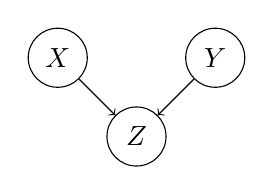
\begin{tikzpicture}[->]
					\node [rv] (X) at (0,  0) {\(X\)};
					\node [rv] (Y) at (2,  0) {\(Y\)};
					\node [rv] (Z) at (1, -1) {\(Z\)};

					\draw (X) to (Z);
					\draw (Y) to (Z);
				\end{tikzpicture}
			\end{center}
			the independence \( X \perp Y \) holds but \( X \perp Y \given Z \) does not. This implies that information can flow from \(X\) to \(Y\) iff \(Z\) is given, i.e., having evidence on either \(X\) or \(Y\) is already sufficient to explain the evidence on \(Z\):
			\begin{equation}
				P(X = x \given Z = z, Y = y) \leq P(X = x \given Z = z).
			\end{equation}
		% end

		\subsection{Representation Theorem}
			All this work on independencies raise the question of whether it is actually worth it: what distributions can be represented using a Bayesian network? And what networks are required to represent a distribution? Also, what other independencies apart from the local Markov assumption are encoded in a network? Some independencies can certainly be derived using the relations presented in \autoref{subsec:condIndependence}. Let \(P\) be the real distribution and let \( I(P) \) be the independencies encoded in the true distribution. Similarly, let \( I_\ell(G) \) be the local independencies (induces by the local Markov assumption) encoded in a graph \(G\). Then the key assumption of Bayesian networks is that
			\begin{equation}
				I_\ell(G) \subseteq I(P).
			\end{equation}
			That is, the local independencies only capture such that are actual present in the true distribution. If this relation holds, \(G\) is said to be an \emph{I-map} (independency map) of \(P\).

			\theorem{The \emph{representation theorem} states that \(G\) if an I-map of \(P\) if and only if \(P\) factorizes according to \(G\) via \eqref{eq:bayesNetJoint}.}

			\paragraph{Proof} % 2.54
				The proof is split into proofing "if" and "only if".

				"if": \todo{Representation Theorem: Proof: "if"}

				"only if": Assume, w.l.o.g., a topological ordering \( X_1, X_2, \dots, X_n \) where \(j < i\) for all children \(X_j\) of some random variable \(X_i\). Applying the chain rule to the joint yields \( P(X_1, X_2, \dots, X_n) = \prod_{i = 1}^{n} P(X_1 \given X_1, X_2, \dots, X_{i - 1}) \). By the topological ordering, \( \Pa(X_1) \subseteq \{ X_1, X_2, \dots, X_{i - 1} \} \) and hence, using the local Markov assumption, \( P(X_i \given X_1, X_2, \dots, X_{i - 1}) = P\bigl(X_1 \given \Pa(X_i) \bigr) \). Therefore, \(P\) factorized according to \eqref{eq:bayesNetJoint}.
			% end
		% end

		\subsection{"Adding Edges Does Not Hurt"}
			\theorem{Let \(G\) be an I-map for \(P\). Then any DAG \(G'\) having the same directed edges as \(G\), then \(G'\) is also an I-map of \(P\).}

			From this theorem it follows that
			\begin{itemize}
				\item \(G'\) is strictly more expressive than \(G\) by capturing more independencies, and
				\item adding edges to \(G\) still results in an I-map.
			\end{itemize}

			\paragraph{Proof Idea} % 2.57
				Let \( I_\ell(G) \subseteq I(P) \). To show that \( I_\ell(G') \subseteq I(P) \) holds, it is enough to show \( I_\ell(G') \subsetneq I_\ell(G) \). Note that is enough to show that this property holds if a single edge is added as adding two edges can be understood as two modifications, resulting in a third graph \(G''\). It therefore follows from \( I_\ell(G'') \subsetneq I_\ell(G') \subseteq I_\ell(G) \) that also \( I_\ell(G'') \subsetneq I_\ell(G) \).

				Let \(X\) and \(Y\) be some random variables of \(G\) such that \( Y \not\in \Pa_G(X) \). Then adding an edge \( Y \to X \) only removes local independencies, but does not induce new ones.

				\todo{Adding Edges Does Not Hurt: Proof}
			% end
		% end
	% end

	\section{Encoded Independencies} % 2.59, 3.2, 3.3, 3.28, 3.29
		So far, only local independencies have been considered. However, a Bayesian network encodes even more dependencies by applying the algebra of conditional independencies (\autoref{subsec:condIndependence}; see \autoref{fig:moreIndependencies} for an example).

		The findings of this section are summarized in \autoref{fig:independencies} which gives an overview of the different variants to getting the set of independencies (read this section first before inspecting the figure).

		\begin{figure}
			\centering
			\begin{tikzpicture}[->]
				\node [rv] (A) {\(A\)};
				\node [rv, right = 1 of A] (B) {\(B\)};
				\node [rv, right = 1 of B] (C) {\(D\)};
				\node [rv, right = 1 of C] (D) {\(D\)};

				\draw (A) to (B);
				\draw (B) to (C);
				\draw (C) to (D);
			\end{tikzpicture}
			\caption[A Bayesian Network Captures More than Local Independencies]{Illustration of a Bayesian network capturing more independencies than induced by the local Markov assumption. In this BN, the local Markov assumption encodes \( I_\ell(G) = \{\, B \perp A \given A, C \perp (A, B) \given B, D \perp (A, B, C) \given C \,\} \). However, also \( A \perp D \given C \) is a captured independency, for example.}
			\label{fig:moreIndependencies}
		\end{figure}

		\begin{figure}
			\centering
			\begin{tikzpicture}[->, box/.style = { draw, rectangle, minimum width = 1.5cm, minimum height = 1.5cm }]
				\node [box] (G) at (0,  0) {\(G\)};
				\node [box] (IG) at (3, -3) {\(I(G)\)};
				\node [box] (IellG) at (3,  0) {\(I_\ell(G)\)};
				\node [box, minimum height = 4.5cm] (IP) at (7.5, -1.5) {\(I(P)\)};
				\path let \p1 = (IP.west), \p2 = (IellG.east) in coordinate(a) at (\x1, \y2);
				\path let \p1 = (IP.west), \p2 = (IG.east) in coordinate(b) at (\x1, \y2);

				\draw (G) to node[above]{Reads} (IellG);
				\draw (G) |- node[left]{d-Separation} (IG);
				\draw (IellG) to node[right]{Algebra of Ind.} (IG);
				\draw (IellG) to node[above]{\(\subseteq\)} (a);
				\draw (IG) to node[above]{\(\subseteq / =\)} (b);
			\end{tikzpicture}
			\caption[Illustration of Independency Capturing]{Illustration of different methods to capture the independencies of a distribution. Note that \(I(G)\) and \(I(P)\) are equal (i.e., \(P\) is faithful to \(G\)) for almost all \(P\) that factor over \(G\).}
			\label{fig:independencies}
		\end{figure}

		\subsection{Dependency Structures}
			In a three-node BN, four types of structures are possible. The first, second, and third are indirect causal and evidential effects and a common cause, respectively:
			\begin{center}
				\begin{tikzpicture}[->]
					\node [rv] (X) {\(X\)};
					\node [rv, right = 1 of X] (Y) {\(Y\)};
					\node [rv, right = 1 of Y] (Z) {\(Z\)};
					\draw (X) to (Y);
					\draw (Y) to (Z);
				\end{tikzpicture}
				\qquad\qquad
				\begin{tikzpicture}[->]
					\node [rv] (X) {\(X\)};
					\node [rv, right = 1 of X] (Y) {\(Y\)};
					\node [rv, right = 1 of Y] (Z) {\(Z\)};
					\draw (Y) to (X);
					\draw (Z) to (Y);
				\end{tikzpicture}
				\qquad\qquad
				\begin{tikzpicture}[->]
					\node [rv] (X) {\(X\)};
					\node [rv, right = 1 of X] (Z) {\(Z\)};
					\node [rv, right = 1 of Z] (Y) {\(Y\)};
					\draw (Z) to (X);
					\draw (Z) to (Y);
				\end{tikzpicture}
			\end{center}
			In both cases, the conditional independence \( X \perp Y \given Z \) holds, but \emph{not} the simple independence \( X \perp Y \).

			The last and most special structure is a v-structure, where two variables have a common effect:
			\begin{center}
				\begin{tikzpicture}[->]
					\node [rv] (X) {\(X\)};
					\node [rv, right = 1 of X] (Z) {\(Z\)};
					\node [rv, right = 1 of Z] (Y) {\(Y\)};
					\draw (X) to (Z);
					\draw (Y) to (Z);
				\end{tikzpicture}
			\end{center}
			In this case, the independencies are inverted: the simple independence \( X \perp Y \) holds, but \( X \perp Y \given Z \) \emph{does not}. This is the same effect as the "explain away" phenomenon / Berkson's paradox (\autoref{subsec:berkson}).
		% end

		\subsection{d-Separation}
			\emph{d-Separation} (dependence separation) is a principled way of finding all independencies modeled by a Bayesian network. The main component are trails. A \emph{trail} is a non-cyclic path \( X_1' \fromto X_2' \fromto \cdots \fromto X_k' \) from one random variable \(X_1'\) to another \(X_k'\). Note that a trail can also be along an edge in opposite order (i.e., the trail itself is undirected) and that every edge and note can only be visited once. For example, the network
			\begin{center}
				\begin{tikzpicture}[->]
					\node [rv] (A) {\(A\)};
					\node [rv, right = 1 of A] (B) {\(B\)};
					\node [rv, below = 1 of A] (C) {\(C\)};
					\node [rv, right = 1 of C] (D) {\(D\)};

					\draw (A) to (B);
					\draw (A) to (C);
					\draw (B) to (D);
					\draw (D) to (C);
				\end{tikzpicture}
			\end{center}
			has the following trails:
			\begin{itemize}
				\item \( A \to B \),\, \( A \to C \from D \from B \);\; \( A \to C \),\, \( A \to B \to D \to C \);\; \( A \to B \to D \),\, \( A \to C \from D \)
				\item \( B \from A \),\, \( B \to D \to C \from A \);\; \( B \from A \to C \),\, \( B \to D \to C \);\; \( B \to D \),\, \( B \from A \to C \from D \)
				\item \( C \from A \),\, \( C \from D \from B \from A \);\; \( C \from A \to B \),\, \( C \from D \from B \);\; \( C \from D \),\, \( C \from A \to B \to D \)
				\item \( D \from B \from A \),\, \( D \to C \from A \);\; \( D \from B \),\, \( D \to C \from A \to B \);\; \( D \to C \),\, \( D \from B \from A \to C \)
			\end{itemize}
			Note that as trails are themselves undirected, the graph itself really has half as many trails, but they are kept for consistency.

			d-Separation now uses these trails to extract independencies. Consider any trail \( X_1' \fromto X_2' \fromto \cdots \fromto X_k' \) between two variables \(X_1'\) and \(X_k'\) this trail is \emph{active} if for each triplet \( X_{i - 1}' \fromto X_i' \fromto X_{i + 1}' \), the following holds:
			\begin{itemize}
				\item \eqmakebox[trails][l]{for \( X_{i - 1} \to X_i \to X_{i + 1} \),}\quad     \(X_i\) is \emph{not observed}.
				\item \eqmakebox[trails][l]{for \( X_{i - 1} \from X_i \from X_{i + 1} \),}\quad \(X_i\) is \emph{not observed}.
				\item \eqmakebox[trails][l]{for \( X_{i - 1} \from X_i \to X_{i + 1} \),}\quad   \(X_i\) is \emph{not observed}.
				\item \eqmakebox[trails][l]{for \( X_{i - 1} \to X_i \from X_{i + 1} \),}\quad   \(X_i\) or one of its descendants \emph{is observed}.
			\end{itemize}
			\theorem{}{Two variables \(X\) and \(Y\) are independent given a set of variables \(\mathcal{Z}\) if there is no active trail between \(X\) and \(Y\) if \(\mathcal{Z}\) are observed. They are said to be \emph{d-separated}. The set of independencies obtained via d-separation is called \(I(G)\).}

			\subsubsection{Soundness}
				\theorem{d-Seperation is \emph{sound}. That is, if \(P\) factorizes over \(G\), then \( I(G) \subseteq I(P) \).}

				This means that d-separation only captured independencies that the true distributions exhibits.

				\paragraph{Proof} % 3.16
					\todo{d-Separation Soundness: Proof}
				% end
			% end

			\subsubsection{Completeness}
				A distribution \(P\) is said to be \emph{faithful} if it does not have independencies that cannot be read from \(G\).

				\theorem{For almost all distributions \(P\) that factorize over \(G\), \( I(G) = I(P) \). "Almost all" means that the possible distributions are a set of measure zero parametrizations of the CPTs.}

				Hence, the Bayesian network is usually sufficient for capturing all independence properties of the distribution! But this only holds for complete independence, but there might be context-specific independencies that are not captured.

				\paragraph{Proof} % 3.18
					\todo{d-Separation Completeness: Proof}
				% end
			% end
		% end

		\subsection{Context-Specific Independence (CSI)}
			As already said, d-separation only captures complete independencies, i.e., once for which
			\begin{equation}
				\forall x, \in \val(X), y \in \val(Y), z \in (Z) : (X = x \perp Y = y \given Z = z)
			\end{equation}
			holds but context-specific independencies,
			\begin{equation}
				\exists x, \in \val(X), y \in \val(Y), z \in (Z) : (X = x \perp Y = y \given Z = z),
			\end{equation}
			are not captured.

			One option for representing CSIs are Tree CPDs. \emph{Tree CPDs} encode a distribution \( P\bigl(X \given \Pa(X) \bigr) \) using a decision-tree like structure, where the paths are an assignment of (a subset of) \( \Pa(X) \) and leaves represent the distributions given the assignments on the path. This way, representation size can be drastically reduced when CSIs are present.

			Another variant where CSIs occur is determinism. While determinism already makes the CPT sparse, it has even greater influences on inference as propagating the zeros often leads to a bunch of new zeros.
		% end

		\subsection{The Bayes' Ball Algorithm} % 3.19
			The \emph{Bayes' ball algorithm} is a algorithmic approach to applying d-separation.
			\todo{Bayes' Ball Algorithm}
		% end
	% end

	\section{SOTA Modal}
		Current state-of-the-art (SOTA) models are often characterized by richness in their local structures (determinism, CSI), massive sizes (thousand of variables), and high connectivity (treewidth, see \autoref{subsec:treewidth}). These developments are enabled by high-level modeling tools (relational and first-order logic), the overall advancement in machine learning, and new application areas (e.g., bioinformatics and sensor networks).

		In these big models, it is a must to exploit local and relational structure!
	% end
% end

\chapter{Inference}
	\emph{Inference} is concerned with answering statistical queries in a probabilistic model. As this summary is on probabilistic model, it is concerned with inference in graphical models. However, inference in Bayesian networks is---in general---pretty hopeless aka. NP-hard (even approximate inference). In practice, however, special structures can be exploited producing many effective (approximate) inference algorithms. This chapter covers exact inference whereas approximate inference is covered later in \autoref{c:approxInference}.

	A general probabilistic query is \( P(X \given e) \) computing some probability given some evidence \(e\). The straightforward way to compute the conditional is to directly use its definition,
	\begin{equation}
		P(X \given e) = \frac{P(X, e)}{P(e)}.
	\end{equation}
	This requires computing the joint distribution and marginalizing out \(X\) to get the normalization factor. In general, such a computation has exponential complexity in the number of random variables!

	For all complexity arguments in the following sections, let \(k\) be the number of configurations of a single random variable, \( k = \lvert \val(X) \rvert \), and assume that all random variables have the same number of values.

	\section{Chain Models}
		The simplest BN to perform efficient exact inference in is a chain model
		\begin{center}
			\begin{tikzpicture}[->]
				\node [rv] (X1) {\(X_1\)};
				\node [rv, right = 1 of X1] (X2) {\(X_2\)};
				\node [rv, right = 1 of X2] (X3) {\(X_3\)};
				\node [rv, draw = white, right = 1 of X3] (Xd) {\(\cdots\)};
				\node [rv, right = 1 of Xd] (Xn) {\(X_n\)};

				\draw (X1) to (X2);
				\draw (X2) to (X3);
				\draw (X3) to (Xd);
				\draw (Xd) to (Xn);
			\end{tikzpicture}
		\end{center}
		that factors as
		\begin{equation}
			P(X_1, X_2, \dots, X_n) = P(X_1) \prod_{i = 2}^{n} P(X_i \given X_{i - 1}).
		\end{equation}
		However, to computing \(P(X_n)\) still requires an exponential number of operations, \( \mathcal{O}(k^n) \):
		\begin{align}
			P(X_n)
				&= \sum_{X_1}^{\marg} \sum_{X_2}^{\marg} \cdots \sum_{X_{n - 1}}^{\marg} P(X_1, X_2, \dots, X_{n - 1}, X_n) \\
				&= \sum_{X_1}^{\marg} \sum_{X_2}^{\marg} \cdots \sum_{X_{n - 1}}^{\marg} P(X_1) \, P(X_2 \given X_1) \, \cdots \, P(X_n \given X_{n - 1}).
		\end{align}
		Instead, it is advisable to reverse the sums and to pull the independent factors out of the marginalization. This corresponds to iteratively computing \( P(X_1) \), \( P(X_2) \), \dots, \( P(X_n) \):
		\begin{equation}
			P(X_{i + 1}) = \sum_{X_i}^{\marg} P(X_{i + 1} \given X_i) \, P(X_i).
		\end{equation}
		This process is linear in the number of random variables and quadratic in the number of values of a random variable, \( \mathcal{O}(nk^2) \)! Hence, at least for simple chain models, inference is tractable.
	% end

	\section{Variable Elimination}
		\label{sec:variableElimination}

		\emph{Variable elimination} extends the idea introduced in the chain models of pulling factors out of the marginalization sums. To incorporate evidence \(e\), the corresponding RVs are simply set to the respective values and marginalization over these variables is removed. See section 8.2.1 in \emph{Data Mining and Machine Learning}\footnote{\url{https://fabian.damken.net/summaries/cs/elective/iws/dmml/dmml-summary.pdf}} for a more thorough treatment of this topic. By convention, the factor that appears by eliminating a variable \(X\) that still depends on other RVs \( Y_1, Y_2, \dots, Y_k \) is named \( f_X(Y_1, Y_2, \dots, Y_k) \). Pseudocode for variable elimination is shown in \autoref{alg:variableElimination}.

		One of the most important steps in variable elimination is pruning the non-active variables (\autoref{algline:vePrune}). This means removing all random variables that are independent of all variables in \( \vec{X} \cup \vec{E} \) as the distributions over these random variables simply reduce to a multiplication with \num{1}, not changing the results. However, this can reduce the number of required operations to a tractable amount.

		The most important aspect determining the efficiency of variable elimination is, intuitively, the choice of the elimination ordering (this is covered in more detail in \autoref{sec:veMoral}). For relatively simple networks like polytrees\footnote{A polytree is the directed variant of a tree. That is, a DAG is a polytree if its underlying undirected graph is a tree.}, inference is linear in \emph{representation} size (i.e., in the number of entries across all CPTs)! In general, however, variable elimination exponential in the number of variables in the intermediate factors---hence its complexity is dominated by the largest intermediate factor. This again is discussed in more detail in \autoref{sec:veMoral}.

		While variable elimination on a general Bayesian network is still exponential in time w.r.t. the number of variables in the intermediate factors, it is linear (in representation size!) in polytree networks.

		Also note that variable elimination can also directly be applied to potentials. It is not required that the original factors actually represent CPTs.

		\begin{algorithm}  \DontPrintSemicolon
			\KwIn{Bayesian network with RVs \( X_1, X_2, \dots, X_n \) and query \( P(\vec{X} \given \vec{E} = \vec{e}) \)}
			\KwOut{Probability \( P(\vec{X} \given \vec{E} = \vec{e}) \)}
			Instantiate evidence \( \vec{E} = \vec{e} \). \;
			Prune non-active variables (w.r.t. \( \vec{X} \cup \vec{E} \)), giving \( X_1, X_2, \dots, X_{\tilde{n}} \), \( \tilde{n} \leq n \).  \label{algline:vePrune} \;
			Choose an ordering \( X_1, X_2, \dots, X_{\tilde{n}} \). \;
			\tcp{Initialize factors:}
			\( \mathcal{F}^{(0)} \gets \bigl\{ f_i = P\bigl( X_i \given \Pa(X_i) \bigr) : i = 1, 2, \dots, \tilde{n} \bigr\} \) \;
			\For{\( i = 1, 2, \dots, \tilde{n} \)}{
				\If{\( X_i \in \vec{X} \cup \vec{E} \)}{
					\textbf{skip} \;
				}
				Collect factors \( f_1, f_2, \dots, f_k \in \mathcal{F}^{(i - 1)} \) containing \(X_i\). \;
				\tcp{Generate a new factor \(g\) by eliminating \(X_i\):}
				\( g = \sum_{X_i}^{\marg} \prod_{i = 1}^{k} f_j \) \;
				\tcp{Replace factors in factor set:}
				\( \mathcal{F}^{(i)} \gets \bigl( \mathcal{F}^{(i - 1)} \setminus \{ f_1, f_2, \dots, f_k \} \bigr) \cup \{ g \} \) \;
			}
			Read only remaining factor \( P(\vec{X}, \vec{E} = \vec{e}) \) from \( \mathcal{F}^{(\tilde{n})} \). \;
			Normalize \( P(\vec{X}, \vec{E} = \vec{e}) \) to get \( P(\vec{X} \given \vec{E} = \vec{e}) \). \;
			\caption{Variable Elimination}
			\label{alg:variableElimination}
		\end{algorithm}
	% end

	\section{Abductive Inference}
		So far, only the calculation of a-posterior beliefs/probabilities has been covered. That is, computing queries of the form \( P(\vec{X} \given \vec{E} = \vec{e}) \) (where \(\vec{E}\) is a, possibly empty, set of evidence). While this type of inference is useful in many cases (e.g., to perform predictions by computing the probability of an outcome, diagnosing a disease by computing the probability given some symptoms, \dots), it is also desirable to perform \emph{abductive} inference. \emph{Abductive inference} is concerned with finding a configuration of a set of random variables that "best" explains the evidence at hand. This can be done in two fashions:
		\begin{itemize}
			\item Most Probable Explanation (MPE): finding the most probable configuration of \emph{all} variables in a Bayesian network given some evidence.
			\item Maximum A Posteriori (MAP): finding the most probable configuration of a \emph{subset} of variables in a Bayesian network given some evidence.
		\end{itemize}
		Note that being able to perform either does not necessarily solve the other (i.e., the MPE cannot be found by individually maximizing all probabilities for all variables and the MAP cannot be found by taking the corresponding subset of the MPE). It is said that MPE and MAP are \emph{not consistent}.

		Finding (approximate) MPEs is quite straightforward by replacing the sums (marginalizations) in variable elimination by \(\max\)'s. In a second backward pass, the sums are replace by \(\argmax\)-operators to find the configuration. A pseudocode version of this approach is given in \autoref{alg:variableEliminationMpe}.

		\begin{algorithm}  \DontPrintSemicolon
			\KwIn{Bayesian network with RVs \( X_1, X_2, \dots, X_n \) and evidence \( \vec{E} = \vec{e} \)}
			\KwOut{Most probable explanation \( \vec{x}^\ast \)}
			Instantiate evidence \( \vec{E} = \vec{e} \). \;
			Prune non-active variables (w.r.t. \( \vec{X} \cup \vec{E} \)), giving \( X_1, X_2, \dots, X_{\tilde{n}} \), \( \tilde{n} \leq n \). \;
			Choose an ordering \( X_1, X_2, \dots, X_{\tilde{n}} \). \;
			\tcp{Initialize factors:}
			\( \mathcal{F}^{(0)} \gets \bigl\{ f_i = P\bigl( X_i \given \Pa(X_i) \bigr) : i = 1, 2, \dots, \tilde{n} \bigr\} \) \;
			\For{\( i = 1, 2, \dots, \tilde{n} \)}{
				\If{\( X_i \in \vec{E} \)}{
					\textbf{skip} \;
				}
				Collect factors \( f_1, f_2, \dots, f_k \in \mathcal{F}^{(i - 1)} \) containing \(X_i\). \;
				\tcp{Generate a new factor \(g\) by maximizing over \(X_i\):}
				\( g = \max_{X_i} \; \prod_{i = 1}^{k} f_j \) \;
				\tcp{Replace factors in factor set:}
				\( \mathcal{F}^{(i)} \gets \bigl( \mathcal{F}^{(i - 1)} \setminus \{ f_1, f_2, \dots, f_k \} \bigr) \cup \{ g \} \) \;
			}
			\tcp{Initilize vector of MPE-values:}
			\( \vec{x}^\ast \in \val(X_1) \times \val(X_2) \times \cdots \times \val(X_n) \) \;
			\For{\( i = \tilde{n}, \tilde{n} - 1, \dots, 1 \)}{
				\If{\( X_i \in \vec{E} \)}{
					\tcp{Copy evident value to result vector:}
					\( x_i^\ast \gets e_i \) \;
				}
				\Else{
					\tcp{Compute \(\argmax\) over \(X_i\), incorporating the evidence and already determined values:}
					\( x_i^\ast \gets \argmax_{X_i} \; \prod_{f \in \mathcal{F}^{i - 1}} f(\vec{x}_{1:i - 1}^\ast, \vec{e}) \) \;
				}
			}
			Set pruned variables \( X_{\tilde{n} + 1}, X_{\tilde{n} + 2}, \dots, X_n \) so arbitrary values. \;
			\caption{Most Probable Explanations via Variable Elimination}
			\label{alg:variableEliminationMpe}
		\end{algorithm}
	% end

	\section{Complexity of Conditional Queries}
		In general, inference on conditional query \( P(\vec{X} \given \vec{E} = \vec{e}) \) is NP-hard. This can be shown by reducing 3-SAT to inference in a Bayesian network. 3-SAT is concerned with the question whether a propositional formula (in conjunctive normal form) with at most three literals per clause is satisfiable. For instance, is the following formula satisfiable (with boolean \(X_1, X_2, \dots, X_4\))?
		\begin{equation}
			\psi = (\lnot X_1 \lor X_2 \lor X_3) \land (X_2 \lor \lnot X_3 \lor X_4) \land (X_1 \lor \lnot X_2)  \label{eqn:3sat}
		\end{equation}
		This problem is known to be NP-hard. This problem can be expressed using a Bayesian network:
		\begin{center}
			\begin{tikzpicture}[->]
				\node [rv]                  (C1) {\(C_1\)};
				\node [rv, right = 1 of C1] (C2) {\(C_2\)};
				\node [rv, right = 1 of C2] (C3) {\(C_3\)};
				\node [rv, right = 1 of C3] (PS) {\(\psi\)};
				\node [rv, above = 0.5 of C1, xshift = 1.75cm/2] (X1) {\(X_1\)};
				\node [rv, above = 0.5 of C2, xshift = 1.75cm/2] (X2) {\(X_2\)};
				\node [rv, below = 0.5 of C1, xshift = 1.75cm/2] (X3) {\(X_3\)};
				\node [rv, below = 0.5 of C2, xshift = 1.75cm/2] (X4) {\(X_4\)};

				\draw (X1) to (C1);
				\draw (X2) to (C1);
				\draw (X3) to (C1);
				\draw (X2) to (C2);
				\draw (X3) to (C2);
				\draw (X4) to (C2);
				\draw (X1) to (C3);
				\draw (X2) to (C3);
				\draw (C1) to (C2);
				\draw (C2) to (C3);
				\draw (C3) to (PS);
			\end{tikzpicture}
		\end{center}
		The CPTs of \(C_1\), \(C_2\), and \(C_3\) then encode the clauses of \eqref{eqn:3sat} and \(\psi\) summarizes them into a single random variable. While it seems possible to just direct all random variables into \(\psi\), this would make the reduction non-polynomial, invalidating the proof of NP-hardness. By putting a prior \( P(X_i = \mathfrak{t}) = 0.5 \) over all (boolean) RVs, satisfiability can be queried as \( P(\psi = \mathfrak{t}) > 0 \). Hence, if conditional inference would be tractable, 3-SAT would be too. By contradiction, this shows that conditional inference is NP-hard.
		\qed

		However, while NP-hard is already pretty hard, it can also be shown that inference is \#P-complete involving counting all satisfying configurations.

		Even though this shows that inference is hard in the general case, it can be solved for problems with special structures (which are very common). For these, efficient (exact) inference algorithms exist.
	% end

	\section{Variable Elimination in Moral Graphs}
		\label{sec:veMoral}

		The induces moral graph of a Bayesian network is an undirected graph where the members of each clique correspond to the domain of a potential in the Bayesian network. To extract the moral graph from a Bayesian network, it might be necessary to introduce moral links to fulfill this (defining) criterion. A \emph{moral link} is be introduced between unconnected parents of a node\footnote{The term "moralizing" has quite outdated origins and refers to the unmorality of "unmarried" parents.}. The rest of the moral graph is then given as the skeleton (i.e., the underlying undirected graph of a DAG) of the network. An example is given in \autoref{fig:moralizing}. More details on why this moral link is necessary are covered in \autoref{sec:towardsMarkovRandomFields}.

		As variable elimination introduces new factors/potentials into the joint probability, these changes have to be reflected in the moral graph after the elimination. If an elimination step introduces a potential with random variables that have not yet been together in a potential, a \emph{fill-in} is introduced to the moral graph representing this new connection. An example of this process is shown in \autoref{fig:fillIns}. An elimination ordering is said to be \emph{perfect} if it does not introduce any fill-ins (see \autoref{fig:perfectSequence} for an example with the same graph used in \autoref{fig:fillIns}).

		\begin{figure}
			\centering
			\begin{subfigure}{0.49\linewidth}
				\centering
				\begin{tikzpicture}[->]
					\node [rv] (X1) {\(X_1\)};
					\node [rv, below left = 1 of X1] (X2) {\(X_2\)};
					\node [rv, below right = 1 of X1] (X3) {\(X_3\)};
					\node [rv, below left = 1 of X2] (X4) {\(X_4\)};
					\node [rv, below right = 1 of X2] (X5) {\(X_5\)};
					\node [rv, below right = 1 of X3] (X6) {\(X_6\)};

					\draw (X1) to (X2);
					\draw (X1) to (X3);
					\draw (X2) to (X4);
					\draw (X2) to (X5);
					\draw (X3) to (X5);
					\draw (X3) to (X6);
				\end{tikzpicture}
				\caption{Bayesian Network}
			\end{subfigure}
			\hfill
			\begin{subfigure}{0.49\linewidth}
				\centering
				\begin{tikzpicture}
					\node [rv] (X1) {\(X_1\)};
					\node [rv, below left = 1 of X1] (X2) {\(X_2\)};
					\node [rv, below right = 1 of X1] (X3) {\(X_3\)};
					\node [rv, below left = 1 of X2] (X4) {\(X_4\)};
					\node [rv, below right = 1 of X2] (X5) {\(X_5\)};
					\node [rv, below right = 1 of X3] (X6) {\(X_6\)};

					\draw (X1) to (X2);
					\draw (X1) to (X3);
					\draw (X2) to (X4);
					\draw (X2) to (X5);
					\draw (X3) to (X5);
					\draw (X3) to (X6);

					\draw [TUDa-9b] (X2) to (X3);
				\end{tikzpicture}
				\caption{Moral Graph}
			\end{subfigure}
			\caption[Example for Moralizing]{Example for creating a moral graph (right) from a Bayesian network (left) by moralizing. All edges are turned into undirected edges and a moral link (depicted in {\color{TUDa-9b} red}) has to be introduced between the "unmarried" parents \(X_2\) and \(X_3\) or \(X_5\).}
			\label{fig:moralizing}
		\end{figure}

		\begin{figure}
			\centering
			\begin{subfigure}{0.49\linewidth}
				\centering
				\begin{tikzpicture}
					\node [rv] (X1) {\(X_1\)};
					\node [rv, below left = 1 of X1] (X2) {\(X_2\)};
					\node [rv, below right = 1 of X1, TUDa-9b] (X3) {\(X_3\)};
					\node [rv, below left = 1 of X2] (X4) {\(X_4\)};
					\node [rv, below right = 1 of X2] (X5) {\(X_5\)};
					\node [rv, below right = 1 of X3] (X6) {\(X_6\)};

					\draw (X1) to (X2);
					\draw [TUDa-9b] (X1) to (X3);
					\draw (X2) to (X4);
					\draw (X2) to (X5);
					\draw [TUDa-9b] (X3) to (X5);
					\draw [TUDa-9b] (X3) to (X6);
					\draw [TUDa-9b] (X2) to (X3);
				\end{tikzpicture}
				\caption{About to eliminate \(X_3\). The affected node and edges are depicted in {\color{TUDa-9b} red}.}
			\end{subfigure}
			\hfill
			\begin{subfigure}{0.49\linewidth}
				\centering
				\begin{tikzpicture}
					\node [rv] (X1) {\(X_1\)};
					\node [rv, below left = 1 of X1] (X2) {\(X_2\)};
					\node [rv, below left = 1 of X2] (X4) {\(X_4\)};
					\node [rv, below right = 1 of X2] (X5) {\(X_5\)};
					\node [rv, below right = 1 of X3] (X6) {\(X_6\)};

					\draw (X1) to (X2);
					\draw (X2) to (X4);
					\draw (X2) to (X5);

					\draw [TUDa-9b] (X1) to (X6);
					\draw [TUDa-9b] (X1) to (X5);
					\draw [TUDa-9b] (X2) to (X6);
					\draw [TUDa-9b] (X5) to (X6);
				\end{tikzpicture}
				\caption{After eliminating \(X_3\). The introduces fill-ins are depicted in {\color{TUDa-9b} red}.}
			\end{subfigure}
			\caption[Example for Elimination in Moral Graphs]{Example for eliminating a variable in a moral graph.}
			\label{fig:fillIns}
		\end{figure}

		\begin{figure}
			\centering
			\begin{subfigure}{0.49\linewidth}
				\centering
				\begin{tikzpicture}
					\node [rv, TUDa-9b] (X1) {\(X_1\)};
					\node [rv, below left = 1 of X1] (X2) {\(X_2\)};
					\node [rv, below right = 1 of X1] (X3) {\(X_3\)};
					\node [rv, below left = 1 of X2] (X4) {\(X_4\)};
					\node [rv, below right = 1 of X2] (X5) {\(X_5\)};
					\node [rv, below right = 1 of X3] (X6) {\(X_6\)};

					\draw [TUDa-9b] (X1) to (X2);
					\draw [TUDa-9b] (X1) to (X3);
					\draw (X2) to (X4);
					\draw (X2) to (X5);
					\draw (X3) to (X5);
					\draw (X3) to (X6);
					\draw (X2) to (X3);
				\end{tikzpicture}
				\caption{About to eliminate \(X_1\).}
			\end{subfigure}
			\hfill
			\begin{subfigure}{0.49\linewidth}
				\centering
				\begin{tikzpicture}
					\node [rv, white] (X1) {\(X_1\)};
					\node [rv, below left = 1 of X1] (X2) {\(X_2\)};
					\node [rv, below right = 1 of X1] (X3) {\(X_3\)};
					\node [rv, below left = 1 of X2, TUDa-9b] (X4) {\(X_4\)};
					\node [rv, below right = 1 of X2] (X5) {\(X_5\)};
					\node [rv, below right = 1 of X3] (X6) {\(X_6\)};

					\draw [white] (X1) to (X2);
					\draw [white] (X1) to (X3);
					\draw [TUDa-9b] (X2) to (X4);
					\draw (X2) to (X5);
					\draw (X3) to (X5);
					\draw (X3) to (X6);
					\draw (X2) to (X3);
				\end{tikzpicture}
				\caption{After eliminating \(X_1\), about to eliminate \(X_4\).}
			\end{subfigure}
			\\
			\begin{subfigure}{0.49\linewidth}
				\centering
				\begin{tikzpicture}
					\node [rv, white] (X1) {\(X_1\)};
					\node [rv, below left = 1 of X1] (X2) {\(X_2\)};
					\node [rv, below right = 1 of X1] (X3) {\(X_3\)};
					\node [rv, below left = 1 of X2, white] (X4) {\(X_4\)};
					\node [rv, below right = 1 of X2] (X5) {\(X_5\)};
					\node [rv, below right = 1 of X3, TUDa-9b] (X6) {\(X_6\)};

					\draw [white] (X1) to (X2);
					\draw [white] (X1) to (X3);
					\draw [white] (X2) to (X4);
					\draw (X2) to (X5);
					\draw (X3) to (X5);
					\draw [TUDa-9b] (X3) to (X6);
					\draw (X2) to (X3);
				\end{tikzpicture}
				\caption{After eliminating \(X_4\), about to eliminate \(X_6\).}
			\end{subfigure}
			\hfill
			\begin{subfigure}{0.49\linewidth}
				\centering
				\begin{tikzpicture}
					\node [rv, white] (X1) {\(X_1\)};
					\node [rv, below left = 1 of X1, TUDa-9b] (X2) {\(X_2\)};
					\node [rv, below right = 1 of X1] (X3) {\(X_3\)};
					\node [rv, below left = 1 of X2, white] (X4) {\(X_4\)};
					\node [rv, below right = 1 of X2] (X5) {\(X_5\)};
					\node [rv, below right = 1 of X3, white] (X6) {\(X_6\)};

					\draw [white] (X1) to (X2);
					\draw [white] (X1) to (X3);
					\draw [white] (X2) to (X4);
					\draw [TUDa-9b] (X2) to (X5);
					\draw (X3) to (X5);
					\draw [white] (X3) to (X6);
					\draw [TUDa-9b] (X2) to (X3);
				\end{tikzpicture}
				\caption{After eliminating \(X_6\), about to eliminate \(X_2\).}
			\end{subfigure}
			\\
			\begin{subfigure}{0.49\linewidth}
				\centering
				\begin{tikzpicture}
					\node [rv, white] (X1) {\(X_1\)};
					\node [rv, below left = 1 of X1, white] (X2) {\(X_2\)};
					\node [rv, below right = 1 of X1, TUDa-9b] (X3) {\(X_3\)};
					\node [rv, below left = 1 of X2, white] (X4) {\(X_4\)};
					\node [rv, below right = 1 of X2] (X5) {\(X_5\)};
					\node [rv, below right = 1 of X3, white] (X6) {\(X_6\)};

					\draw [white] (X1) to (X2);
					\draw [white] (X1) to (X3);
					\draw [white] (X2) to (X4);
					\draw [white] (X2) to (X5);
					\draw [TUDa-9b] (X3) to (X5);
					\draw [white] (X3) to (X6);
					\draw [white] (X2) to (X3);
				\end{tikzpicture}
				\caption{After eliminating \(X_2\), about to eliminate \(X_3\).}
			\end{subfigure}
			\hfill
			\begin{subfigure}{0.49\linewidth}
				\centering
				\begin{tikzpicture}
					\node [rv, white] (X1) {\(X_1\)};
					\node [rv, below left = 1 of X1, white] (X2) {\(X_2\)};
					\node [rv, below right = 1 of X1, white] (X3) {\(X_3\)};
					\node [rv, below left = 1 of X2, white] (X4) {\(X_4\)};
					\node [rv, below right = 1 of X2] (X5) {\(X_5\)};
					\node [rv, below right = 1 of X3, white] (X6) {\(X_6\)};

					\draw [white] (X1) to (X2);
					\draw [white] (X1) to (X3);
					\draw [white] (X2) to (X4);
					\draw [white] (X2) to (X5);
					\draw [white] (X3) to (X5);
					\draw [white] (X3) to (X6);
					\draw [white] (X2) to (X3);
				\end{tikzpicture}
				\caption{After eliminating \(X_3\), elimination finished.}
			\end{subfigure}
			\caption[Example for a Perfect Elimination Sequence]{Example for a perfect elimination sequence executed in a moral graph. The variable that should be eliminated is always depicted in {\color{TUDa-9b} red} and is eliminated in the upcoming graph.}
			\label{fig:perfectSequence}
		\end{figure}

		\subsection{Complexity}
			As already pointed out in \autoref{sec:variableElimination}, the driving factor of the complexity of VE is the number of variables in the intermediate factors. Hence, for VE on moral graphs, the complexity is determined by the number of variables in the domains of the potentials producing during the elimination. This leads to a set of domains where all sets that are subsets of other sets can be removed (as they do not affect the complexity). For the elimination ordering shown in \autoref{fig:perfectSequence}, these are, in order of appearance, the following sets:
			\begin{align}
				&\bigl\{ \{ X_1, X_2, X_3 \},\, \{ X_2, X_4 \}, \{ X_3, X_6 \}, \{ X_2, X_3, X_5 \}, \{ X_3, X_5 \}, \{ X_5 \} \bigr\} \\
				\longrightarrow\qquad
				&\bigl\{ \{ X_1, X_2, X_3 \},\, \{ X_2, X_4 \}, \{ X_3, X_6 \}, \{ X_2, X_3, X_5 \} \bigr\}
			\end{align}
			It turns out that all perfect elimination orderings (i.e., those that do not produce fill-ins), have the same set of potential domains. Also, all perfect elimination orderings ending some random variable \(X\) are \emph{optimal} in terms of computing \( P(X) \).

			For the imperfect elimination ordering \( (X_3, X_4, X_6, X_1, X_2, X_5) \) (for which the first elimination is shown in \autoref{fig:fillIns}), the following sets of potentials are created:
			\begin{align}
				&\bigl\{ \{ X_1, X_2, X_3, X_5, X_6 \},\, \{ X_2, X_4 \}, \{ X_1, X_2, X_5, X_6 \}, \{ X_1, X_2, X_5 \}, \{ X_2, X_5 \}, \{ X_5 \} \bigr\} \\
				\longrightarrow\qquad
				&\bigl\{ \{ X_1, X_2, X_3, X_5, X_6 \},\, \{ X_2, X_4 \} \bigr\}
			\end{align}
			Intuitively, the number of items of this clique are closely related to the complexity of VE (a small clique set corresponds to large connectivity in the graph, hence large factors).

			\subsubsection{Induced Graph and Treewidth}
				To further formalize the aforementioned idea, the notion of an induced graph is introduced. The \emph{induced graph} of some moral graph is the graph including all connections of the clique set, i.e., the moral graph with all fill-ins inserted. Hence, the moral graph is also a sub-graph of the induced graph. For the perfect elimination ordering of \autoref{fig:perfectSequence}, the induced graph is also the moral graph (as no fill-ins were added). However, for the imperfect elimination sequence \( (X_3, X_4, X_6, X_1, X_2, X_5) \), the induced graph has more connections as shown in \autoref{fig:imperfectInducedGraph}.

				It is clear that the size of the maximum clique differs for the perfect and imperfect elimination sequence. This quantity (minus one) is called the \emph{treewidth} of a graph and is called \emph{induced} treewidth for a Bayesian network combined with an elimination ordering (which highly influences the treewidth of the moral graph). Hence, finding a good elimination ordering is equivalent to minimizing the treewidth of the induced graph.

				\begin{figure}
					\centering
					\begin{tikzpicture}
						\node [rv] (X1) {\(X_1\)};
						\node [rv, below left = 1 of X1] (X2) {\(X_2\)};
						\node [rv, below right = 1 of X1] (X3) {\(X_3\)};
						\node [rv, below left = 1 of X2] (X4) {\(X_4\)};
						\node [rv, below right = 1 of X2] (X5) {\(X_5\)};
						\node [rv, below right = 1 of X3] (X6) {\(X_6\)};

						\draw (X1) to (X2);
						\draw (X1) to (X3);
						\draw (X2) to (X4);
						\draw (X2) to (X5);
						\draw (X3) to (X5);
						\draw (X3) to (X6);
						\draw (X2) to (X3);

						\draw (X1) to[bend left] (X6);
						\draw (X1) to (X5);
						\draw (X2) to (X6);
						\draw (X5) to (X6);
					\end{tikzpicture}
					\caption[Induced Graph for Imperfect Elimination Ordering]{Induced graph for the imperfect elimination ordering \( (X_3, X_4, X_6, X_1, X_2, X_5) \).}
					\label{fig:imperfectInducedGraph}
				\end{figure}
			% end

			\subsubsection{(Poly-) Trees}
				A direct consequence of the tight coupling between the complexity of VE and the treewidth is that inference on a "tree" Bayesian network (one in which every node has at most one parent) is linear in the number of variables (as the treewidth is \num{1} for a tree)! Finding an elimination ordering is also straightforward: by starting from the leaves, each factor only involves two RVs. It is also guaranteed that a tree has a leave, so the ordering cannot stall.

				For polytree Bayesian networks (ones of which the skeleton is a tree but a node may have more than one parent), the treewidth is \num{2} and inference is linear in CPT size (i.e., representation size of the network). Opposed to a tree BN, the treewidth \emph{is not} \num{1} as moral links have to be added between "unmarried" parents.
			% end

			\subsubsection{General Networks}
				For general networks, the treewidth is usually greater than \num{1}. In fact, for any graph that has a cycle, the treewidth is at least \num{2}. Form graph theory, it is known that finding an optimal ordering minimizing the treewidth is NP-hard, so again, in general, inference is intractable. However, there are some neat heuristics that can be applied for finding "good" (but not necessarily optimal) orderings. There also exist algorithm that---if the graph has low treewidth---find the optimal ordering in polynomial time. Also, incorporating CSIs can reduce the complexity to be tractable even for graphs with large treewidth.

				A summary of the complexity results is given in \autoref{fig:inferenceComplexity}.

				\begin{table}
					\centering
					\begin{tabular}{c|c|c}
						\toprule
						                                &          \multicolumn{2}{c}{\textbf{Graph Type}}          \\
						        \textbf{Query}          &         \textbf{General}         & \textbf{Low Treewidth} \\ \midrule
						    Probabilistic Inference     &           \#P-Complete           &          Easy          \\
						Most Probable Explanation (MPE) &           NP-Complete            &          Easy          \\
						  Maximum A Posteriori (MAP)    & \(\text{NP}^\text{PP}\)-Complete &        NP-Hard         \\ \bottomrule
					\end{tabular}
					\begin{center}
						For approximate probabilistic inference, hardness depends on the error: \\
						\eqmakebox[complexSummaryA][r]{Absolute Error, \( \lvert \hat{P} - P \rvert \leq \epsilon \):\quad}
						\eqmakebox[complexSummaryB][l]{NP-Hard for \( \epsilon < 0.5 \)} \\
						\eqmakebox[complexSummaryA][r]{Relative Error, \( \lvert \hat{P} - P \rvert / P \leq \epsilon \):\quad}
						\eqmakebox[complexSummaryB][l]{NP-Hard for \( \epsilon > 0 \)}
					\end{center}
					\vspace{-0.4cm}
					\caption[Summary of Inference Complexities]{Summary of complexities for various inference queries.}
					\label{fig:inferenceComplexity}
				\end{table}
			% end
		% end
	% end
% end

\chapter{Markov Random Fields}
	Bayesian networks are not allowed to have cycles as they would not make any sense. Another variant of PGMs, Markov Random Fields (MRFs), allow cycles and are undirected. Instead of encoding dependencies, the edges in a Markov network encode which random variables occur together in a potential. For example, the Markov network
	\begin{center}
		\begin{tikzpicture}
			\node [rv] (X1) {\(X_1\)};
			\node [rv, right = 1 of X1] (X2) {\(X_2\)};
			\node [rv, right = 1 of X2] (X3) {\(X_3\)};
			\node [rv, below = 1 of X2] (X4) {\(X_4\)};
			\node [rv, below = 1 of X3] (X5) {\(X_5\)};
			\draw (X1) to (X2);
			\draw (X2) to (X3);
			\draw (X2) to (X4);
			\draw (X3) to (X5);
			\draw (X4) to (X5);
		\end{tikzpicture}
	\end{center}
	corresponds to the distribution
	\begin{equation}
		P(X_1, X_2, X_3, X_4, X_5) \propto \phi(X_1, X_2) \, \phi(X_2, X_3) \, \phi(X_2, X_4) \, \phi(X_3, X_5) \, \phi(X_4, X_5)
	\end{equation}
	up to normalization. In general, a distribution \( P(X_1, X_2, \dots, X_n) \) specified by a MRF \(G\) factors as
	\begin{equation}
		P(X_1, X_2, \dots, X_n) = \frac{1}{Z} \prod_{C \,\in\, \Cliques(G)} \phi_C(X_1, X_2, \dots, X_n)
	\end{equation}
	where \( \Cliques(G) \) is the set of maximal cliques in \(G\) and \(1/Z\) is the normalization factor. In an MRF, the \emph{Markov property} holds: two sets of random variables, \(\mathcal{X}\) and \(\mathcal{Y}\) are independent given a \emph{separating subset} \(\mathcal{Z}\) (\( \mathcal{X} \perp \mathcal{Y} \given \mathcal{Z} \)). This subset has the property that every path from any variable in \(\mathcal{X}\) to any variable in \(\mathcal{Y}\) contains a variable from \(\mathcal{Z}\).

	\paragraph{Proof}
		\todo{Proof of Markov Property in MRFs}
	% end

	\section{Bayesian Networks as MRFs}
		\label{sec:towardsMarkovRandomFields}

		It is possible to convert Bayesian networks into MRFs for leveraging the theory that evolved around them. This process was already introduced as \emph{moralizing} before (\autoref{sec:veMoral}).	 This section builds up a more formal view on how the addition of a moral link is necessary. The following paragraphs show to convert the fundamental building blocks (pair, chain, common cause, and common effect) of a Bayesian network into a Markov network.

		\paragraph{Pair}
			\begin{center}
				\begin{tikzpicture}
					\node [rv] (X1) {\(X\)};
					\node [rv, right = 1 of X1] (Y1) {\(Y\)};
					\draw [->] (X1) to (Y1);

					\node [right = 2 of Y1] (a) {\(\longrightarrow\)};

					\node [rv, right = 2 of a] (X2) {\(X\)};
					\node [rv, right = 1 of X2] (Y2) {\(Y\)};
					\draw (X2) to (Y2);
				\end{tikzpicture}
			\end{center}
			This conversion makes sense as from the Bayesian model,
			\begin{equation}
				P(X, Y) = P(X) \, P(Y \given X),
			\end{equation}
			and from the Markov network,
			\begin{equation}
				P(X, Y) \propto \phi(X, Y)
			\end{equation}
			with \( \phi(X, Y) \propto P(X) \, P(Y \given X) \).
		% end

		\paragraph{Chain}
			\begin{center}
				\begin{tikzpicture}
					\node [rv] (X1) {\(X\)};
					\node [rv, right = 1 of X1] (Y1) {\(Y\)};
					\node [rv, right = 1 of Y1] (Z1) {\(Z\)};
					\draw [->] (X1) to (Y1);
					\draw [->] (Y1) to (Z1);

					\node [right = 2 of Z1] (a) {\(\longrightarrow\)};

					\node [rv, right = 2 of a] (X2) {\(X\)};
					\node [rv, right = 1 of X2] (Y2) {\(Y\)};
					\node [rv, right = 1 of Y2] (Z2) {\(Z\)};
					\draw (X2) to (Y2);
					\draw (Y2) to (Z2);
				\end{tikzpicture}
			\end{center}
			Like for the pair of variables, the joint probability is
			\begin{equation}
				P(X, Y, Z) = P(X) \, P(Y \given X) \, P(Z \given Y)
			\end{equation}
			by the Bayesian model and
			\begin{equation}
				P(X, Y, Z) \propto \phi(X, Y) \, \phi(Y, Z)
			\end{equation}
			by the Markov network with \( \phi(X, Y) \propto P(X) \, P(Y \given X) \) and \( \phi(Y, Z) \propto P(Z \given Y) \). Note that the parametrization of the potentials is not unique.
		% end

		\paragraph{Common Cause}
			\begin{center}
				\begin{tikzpicture}
					\node [rv] (X1) {\(X\)};
					\node [rv, right = 1 of X1] (Y1) {\(Y\)};
					\node [rv, right = 1 of Y1] (Z1) {\(Z\)};
					\draw [->] (Y1) to (X1);
					\draw [->] (Y1) to (Z1);

					\node [right = 2 of Z1] (a) {\(\longrightarrow\)};

					\node [rv, right = 2 of a] (X2) {\(X\)};
					\node [rv, right = 1 of X2] (Y2) {\(Y\)};
					\node [rv, right = 1 of Y2] (Z2) {\(Z\)};
					\draw (Y2) to (X2);
					\draw (Y2) to (Z2);
				\end{tikzpicture}
			\end{center}
			For a common cause, the conversion is again similar to the chain model. By the Bayesian network,
			\begin{equation}
				P(X, Y, Z) = P(X \given Y) \, P(Y) \, P(Z \given Y)
			\end{equation}
			and by the Markov network,
			\begin{equation}
				P(X, Y, Z) \propto \phi(X, Y) \, \phi(Y, Z)
			\end{equation}
			with \( \phi(X, Y) \propto P(X \given Y) \, P(Y) \) and \( \phi(Y, Z) \propto P(Z \given Y) \). Note again that the parametrization is not unique.
		% end

		\paragraph{Common Effect}
			\begin{center}
				\begin{tikzpicture}
					\node [rv] (X1) {\(X\)};
					\node [rv, right = 1 of X1] (Y1) {\(Y\)};
					\node [rv, right = 1 of Y1] (Z1) {\(Z\)};
					\draw [->] (X1) to (Y1);
					\draw [->] (Z1) to (Y1);

					\node [right = 2 of Z1] (a) {\(\longrightarrow\)};

					\node [rv, right = 2 of a] (X2) {\(X\)};
					\node [rv, right = 1 of X2] (Y2) {\(Y\)};
					\node [rv, right = 1 of Y2] (Z2) {\(Z\)};
					\draw (X2) to (Y2);
					\draw (Z2) to (Y2);
					\draw [TUDa-9b] (X2) to[bend left] (Z2);
				\end{tikzpicture}
			\end{center}
			For the v-structure, the conversion is a tad more complicated. By the Bayesian network,
			\begin{equation}
				P(X, Y, Z) = P(X) \, P(Y \given X, Z) \, P(Z).
			\end{equation}
			But if the moral link (depicted in {\color{TUDa-9b} red}) would not be present, the Markov network would model the distribution as
			\begin{equation}
				P(X, Y, Z) = \phi(X, Y) \, P(Y, Z).
			\end{equation}
			However, this would entail \( X \perp Y \given Z \) which is---prominently as Berkson's paradox---not true. Hence, a moral link has to be included to ensure that the said conditional independency does not hold. With the moral link, the Markov network entails
			\begin{equation}
				P(X, Y, Z) \propto \phi(X, Y) \, \phi(Y, Z) \, \phi(X, Z).
			\end{equation}
			Note that this formulation \emph{does not} encode the same independencies: in the Markov network formulation, \( X \perp Y \) does not hold anymore. However, it is more important to not capture invalid independencies than missing out on some.

			This observation depends on the fact that two variables \(X\) and \(Y\) are conditionally dependent given \(Z\) if and only if their distribution \( P(X, Y, Z) \) can be written as \( P(X, Y, Z) = \phi(X, Y) \, \phi(Y, Z) \) with some \(\phi(\cdot)\).
			\todo{Proof}
		% end
	% end

	\section{Triangulated Graphs and Simplicial Nodes}
		For the upcoming sections, some nomenclature is needed:
		\begin{itemize}
			\item A graph is \emph{triangulated} if it has a perfect elimination ordering (i.e., one that does not introduce any fill-inds).
			\item A node is \emph{simplicial} if its family (itself in addition to its neighbors) is equivalent to its maximum clique.
		\end{itemize}
		It follows that in a triangulated graph, the elimination of a simplicial node again yields a triangulated graph. Also, every triangulated graph (with at least two nodes) has at least two simplicial nodes. Hence, it directly follows that a perfect elimination ordering exists for every random variable in the graph.

		Note that it is possible to triangulate every graph by applying any elimination ordering and consider the induced graph instead. However, while this creates a triangulated graph, it does not induce high-performance inference as the produces graph might have very large treewidth!
	% end

	\section{Join Trees}
		A \emph{join tree} is a special kind of tree where each node (also called \emph{cluster} in join trees) holds a set of variables. Additionally, the \emph{running intersection property} (RIP) holds: for each pair of nodes, \(\mathcal{X}\) and \(\mathcal{Y}\), each node along each path between the two nodes contains the intersection \( \mathcal{X} \cap \mathcal{Y} \). An example is shown in \autoref{fig:joinTree}. It can be shown that if the (maximum) cliques of a undirected graph can be organized into a join tree, then the graph is triangulated and vice versa.

		\begin{figure}
			\centering
			\begin{subfigure}{0.49\linewidth}
				\resizebox{\linewidth}{!}{
					\begin{tikzpicture}[every node/.style = { draw, ellipse }]
						\node (a1) {\( \{ B, C, D, E \} \)};
						\node [below left = 1 of a1] (a2) {\( \{ A, B, C, D \} \)};
						\node [below right = 1 of a1] (a3) {\( \{ D, E, F, I \} \)};
						\node [below = 1.5 of a1] (a4) {\( \{ B, C, D, G \} \)};
						\node [below = 1 of a4] (a5) {\( \{ C, H, G, J \} \)};

						\draw (a1) to (a2);
						\draw (a1) to (a3);
						\draw (a1) to (a4);
						\draw (a4) to (a5);
					\end{tikzpicture}
				}
				\caption{Join Tree}
			\end{subfigure}
			\hfill
			\begin{subfigure}{0.49\linewidth}
				\resizebox{\linewidth}{!}{
					\begin{tikzpicture}[every node/.style = { draw, ellipse }]
						\node (a1) {\( \{ B, C, D, E \} \)};
						\node [below left = 1 of a1] (a2) {\( \{ A, B, C, D \} \)};
						\node [below right = 1 of a1] (a3) {\( \{ D, E, F, I \} \)};
						\node [below = 1.5 of a1] (a4) {\( \{ B, C, D, G \} \)};
						\node [below = 1 of a4] (a5) {\( \{ C, H, G, J \} \)};

						\draw (a1) to (a2);
						\draw (a1) to (a3);
						\draw (a3) to (a4);
						\draw (a4) to (a5);
					\end{tikzpicture}
				}
				\caption{No Join Tree}
			\end{subfigure}
			\caption[Join Tree Illustration]{Illustration of a join tree. The left is a join tree, but the right is not as on the path between \( \{ A, B, C, D \} \) and \( \{ C, H, G, J \} \) has to contain \( \{ C \} \) in every node, which is not a subset of \( \{ D, E, F, I \} \).}
			\label{fig:joinTree}
		\end{figure}

		\subsection{Markov Network as a Join Tree: Junction Tree}
			Organizing a triangulated graph into a join tree is straightforward by exploiting the special properties of such a graph. Pseudocode for this process is given in \autoref{alg:triangulatedToJoin} and. A join tree \(G_J\) built from a Markov network \(G'\) also models the joint distribution as
			\begin{equation}
				P(X_1, X_2, \dots, X_n) = \frac{\prod_{C \,\in\, \Cliques(G_J)} \phi_C(X_1, X_2, \dots, X_n)}{\prod_{S \,\in\, \Sep(G_j)} \phi_S(X_1, X_2, \dots, X_n)}
			\end{equation}
			That is, the joint distribution is the product of the clique potentials divided by the product of the separator potentials.

			\begin{algorithm}  \DontPrintSemicolon
				\KwIn{Triangulated undirected graph \(G\) with random variables \( X_1, X_2, \dots, X_n \)}
				\KwOut{Join tree with clique and separator nodes}
				Initialize set of nodes \(\mathcal{X}\). \;
				Initialize count of eliminated nodes \( n \gets 0 \) \;
				\While{\( \mathcal{X} \) is not empty}{
					Pop simplicial node \(X\) from \(\mathcal{X}\). \;
					\tcp{Construct set of variables to eliminate:}
					\( \mathcal{E} \gets \bigl\{ Y \in \Family(X) : \Family(Y) \subseteq \Family(X) \bigr\} \). \;
					Eliminate all variables in \( \mathcal{E} \). \;
					\tcp{Increment counter for number of eliminated variables:}
					\( n \gets n + \lvert \mathcal{E} \rvert \) \;
					\tcp{Create clique and seperator nodes for \(X\):}
					\( V_n \gets \Family(X) \) \;
					\( S_n \gets \Family(X) \setminus \mathcal{E} \) \;
					Connect \( V_n \) and \( S_n \). \;
				}
				Connect each separator \(S_i\) to \emph{exactly one} clique \(V_j\) with \(j > i\) and \( S_i \subseteq V_j \).
				\caption{Triangulated, Undirected Graph \(\to\) Join Tree}
				\label{alg:triangulatedToJoin}
			\end{algorithm}

			\paragraph{Proof}
				\todo{Join Tree Factoring: Proof}
			% end
		% end
	% end

	\section{Junction Trees}
		\label{sec:junctionTrees}

		A \emph{junction tree} of a Markov network is a join tree for which each factor \(\phi\) in the Markov network is associated to a cluster \(V\) in the join tree such that \( \dom \phi \subseteq V \). This is called the \emph{family preservation property} of junction trees. Such a join tree can, for example, be generated using \autoref{alg:triangulatedToJoin} if an elimination ordering is given; see \autoref{fig:junctionTree} for an example. However, it is not necessary to build up a triangulated graph beforehand in general (it would be, for example, possible to create a junction tree with a node containing all nodes of the original tree; however, this would be useless as it does not leverage any theory of junction trees at all).

		Ideally, the clusters are as small and modular as possible. Unfortunately, it is NP-hard to find the optimal tree\dots However, some useful heuristics and special cases exists. For example, tree-BNs can directly be converted to an efficient junction tree by converting each edge into a cluster.

		\begin{figure}
			\centering
			\begin{subfigure}{0.4\linewidth}
				\centering
				\begin{tikzpicture}
					\node [rv] (X1) {\(X_1\)};
					\node [rv, below left = 1 of X1] (X2) {\(X_2\)};
					\node [rv, below right = 1 of X1] (X3) {\(X_3\)};
					\node [rv, below left = 1 of X2] (X4) {\(X_4\)};
					\node [rv, below right = 1 of X2] (X5) {\(X_5\)};
					\node [rv, below right = 1 of X3] (X6) {\(X_6\)};

					\draw (X1) to (X2);
					\draw (X1) to (X3);
					\draw (X2) to (X4);
					\draw (X2) to (X5);
					\draw (X3) to (X5);
					\draw (X3) to (X6);
					\draw (X2) to (X3);
				\end{tikzpicture}
				\caption{Markov Network}
			\end{subfigure}
			\hfill
			\begin{subfigure}{0.59\linewidth}
				\centering
				\begin{tikzpicture}[align = center]
					\node [fam] (V6) {\( V_6 \) \\ \( \{ X_2, X_3, X_5 \} \)};
					\node [sep, left  = 2.5 of V6.south, yshift = -0.75cm, anchor = north east] (S1) {\( S_1 \) \\ \( \{ X_2, X_3 \} \)};
					\node [sep, below = 0.75 of V6.south, anchor = north] (S2) {\( S_2 \) \\ \( \{ X_2 \} \)};
					\node [sep, right = 2.5 of V6.south, yshift = -0.75cm, anchor = north west] (S3) {\( S_3 \) \\ \( \{ X_3 \} \)};
					\node [fam, below = 1 of S1] (V1) {\( V_1 \) \\ \( \{ X_1, X_2, X_3 \} \)};
					\node [fam, below = 1 of S2] (V2) {\( V_2 \) \\ \( \{ X_2, X_4 \} \)};
					\node [fam, below = 1 of S3] (V3) {\( V_3 \) \\ \( \{ X_3, X_6 \} \)};

					\draw (V1) to (S1);
					\draw (V2) to (S2);
					\draw (V3) to (S3);
					\draw (S1) |- (V6);
					\draw (S2) to (V6);
					\draw (S3) |- (V6);
				\end{tikzpicture}
				\caption{Junction Tree}
			\end{subfigure}
			\caption[Example of a Junction Tree]{Example of the junction tree (right) produced using \autoref{alg:triangulatedToJoin} with the elimination ordering \( (X_1, X_4, X_6, X_2, X_3, X_5) \) showed in \autoref{fig:perfectSequence}.}
			\label{fig:junctionTree}
		\end{figure}

		\subsection{Inference}
			To perform inference in a junction tree, each node sends exactly one \emph{message} to exactly one of its neighbors once it has received messages from all its other neighbors. Hence, message passing must start at the leaves of the tree. To define a leave, however, first an arbitrary root node must be picked. Messages are then collected at this node and afterwards distributed back across the tree to the leaves. After this process, all clusters have the relevant information to compute the potential for its variables.

			To pass messages between the clusters, each separator \(S_i\) has two "mailboxes" \( \psi_i \) and \( \psi^i \), one for the forward- and one for the backward-pass, respectively. That is, \(\psi_i\) is filled when the messages flow from the leaves to the root while \(\psi^i\) is filled when the beliefs flow back from the root to the leaves. Note that from the construction of the junction tree, each separator has exactly two connections. Each clique \( C_i \) is associated with the potentials \( \phi_j \) of the Markov network for which \( \dom \phi_j \subseteq C_i \) holds. Let \( \Phi(C_i) \) be the set of potentials associated with \(C_i\). Additionally, each clique \(C_i\) is associated with a potential \(\varphi_i\) that is used to store the current belief over the variables of the clique. All of this is illustrated in \autoref{fig:junctionTreeInference}.

			\begin{algorithm}
				\KwIn{Junction tree with separators \( \{ S_j \} \) and cliques \( \{ V_i \} \) with associated potentials \( \Phi(C_i) \) from the Markov network}
				\KwOut{Potentials \( \{ \varphi_j \} \) for each clique}
				Initialize separator potentials
			\end{algorithm}

			\todo{IMPORTANT: Look again at message passing in junction trees! Also consider changing the separator's potentials to phis.}

			\begin{figure}
				\centering
				\begin{tikzpicture}[->, align = center]
					\node [fam] (V6) {
						\( V_6 = \{ X_2, X_3, X_5 \} \) \\
						\( \varphi_6;\; \)
					};
					\node [sep, left  = 2.5 of V6.south, yshift = -0.75cm, anchor = north east] (S1) {
						\( S_1 = \{ X_2, X_3 \} \) \\
						\( \downarrow\; \psi_1 \quad \uparrow\; \psi^1 \)
					};
					\node [sep, below = 0.75 of V6.south, anchor = north] (S2) {
						\( S_2 = \{ X_2 \} \) \\
						\( \downarrow\; \psi^2 \quad \uparrow\; \psi_2 \)
					};
					\node [sep, right = 2.5 of V6.south, yshift = -0.75cm, anchor = north west] (S3) {
						\( S_3 = \{ X_3 \} \) \\
						\( \downarrow\; \psi^3 \quad \uparrow\; \psi_3 \)
					};
					\node [fam, below = 1 of S1] (V1) {
						\( V_1 = \{ X_1, X_2, X_3 \} \) \\
						\( \varphi_1;\; \)
					};
					\node [fam, below = 1 of S2] (V2) {
						\( V_2 = \{ X_2, X_4 \} \) \\
						\( \varphi_2;\; \)
					};
					\node [fam, below = 1 of S3] (V3) {
						\( V_3 = \{ X_3, X_6 \} \) \\
						\( \varphi_3;\; \)
					};

					\draw (S1) to (V1);
					\draw (V2) to (S2);
					\draw (V3) to (S3);
					\draw (V6) -| (S1);
					\draw (S2) to (V6);
					\draw (S3) |- (V6);
				\end{tikzpicture}
				\caption[Messages Boxes used in Junction Tree Message Passing]{Illustration of the message boxes and potentials used for message passing in junction trees, based on the junction tree shown in \autoref{fig:junctionTree}. For this tree, \(V_1\) is chosen as the root node. The arrow directions depict the forward pass, the backward pass goes in reverse.}
				\label{fig:junctionTreeInference}
			\end{figure}
		% end
	% end
% end

\chapter{Learning}
	Until now, it was assumed that both the network structure and the CPTs are given somehow. This chapter is concerned with learning these from data. It is important to be able to learn structures from data as usually, no expert is available that can craft a network by hand or she is really expensive. And in the age of big data, data is cheap and huge amounts of data are available.

	Learning Bayesian network is especially appealing as detecting and modeling conditional independencies captures the structure of many real-world distributions and can lead to knowledge discovery by capturing causal relationships. Also, the learned model can be used for handling missing data and hidden variables.

	In a \emph{complete} dataset, every data point has the values for all attributes that are getting investigated. On the other hand, \emph{incomplete} datasets lack some values of random variables (this is usually the case in real-world data\dots). Also, a special kind of incompleteness, are hidden variables. \emph{Hidden variables} never have assigned values in the whole dataset. One example for this is the cluster ID in an unsupervised clustering problem. They can also present a low-dimensional embedding that summarizes some other variables and separates them from a second set of RVs (dimensionality reduction).

	The relation of the different problem types are summarized in \autoref{tab:learningProblems}.

	\begin{table}
		\centering
		\begin{tabular}{c|ccc}
			\toprule
			\textbf{Observed} & \textbf{Fixed Structure} & \textbf{Fixed Variables} & \textbf{Hidden Variables} \\ \midrule
			\textbf{Fully} & Easy (Counting, MLE) & Selection of Edges & --- \\
			\textbf{Partially} & \makecell{Numerical Optimization \\ (difficult for large networks)} & \makecell{Encompasses for Difficult Subproblem \\ (only structural EM known)} & \makecell{Scientific \\ Discovery} \\ \bottomrule
		\end{tabular}
		\caption[Overview Over Different Learning Problems]{Overview over different learning problems and solution approaches.}
		\label{tab:learningProblems}
	\end{table}

	\section{Parameter Estimation}
		In \emph{parameter estimation}, it is assumed that the structure of the Bayesian network (i.e., the random variables and dependencies between them) is fixed and only the entries of the CPTs have to be estimated. This field further subdivides into the cases of complete and incomplete data.

		\subsection{Known Structure, Complete Data}
			With known structure and complete data, the problem simply reduces to basically counting. The most basic method to do so are maximum likelihood estimators (where the likelihood can be computed using the Bayesian network). Some advantages of ML estimated are that they are (often) intuitive, consistent (the estimate converges to the best possible value with increasing number of data points), and asymptotic efficiency (given a dataset, the estimate is as close as possible to the true value).

			\subsubsection{Decomposability of the Likelihood}
				An important property of the likelihood for a Bayesian network is that it is \emph{decomposable}. Let \( \theta_i \) be the CPT of \( P\bigl(X_i \given \Pa(X_i) \bigr) \) and let \( \vec{x}^{(1)}, \vec{x}^{(2)}, \dots, \vec{x}^{(N)} \) be the data points. Then the log-likelihood is
				\begin{equation}
					\log P(\vec{x}^{(1)}, \vec{x}^{(2)}, \dots, \vec{x}^{(N)} \given \theta_1, \theta_2, \dots, \theta_n)
						= \sum_{j = 1}^{N} \log P(\vec{x}^{(j)} \given \theta_j)
						= \sum_{j = 1}^{N} \sum_{i = 1}^{n} \log P\bigl(X_i = x_i^{(j)} \biggiven \Pa(X_i), \theta_j \bigr).
				\end{equation}
				By swapping the sums, the log-likelihood can be rewritten as
				\begin{equation}
					\log P(\vec{x}^{(1)}, \vec{x}^{(2)}, \dots, \vec{x}^{(N)} \given \theta_1, \theta_2, \dots, \theta_n)
						= \sum_{i = 1}^{n} \log P(\vec{x}^{(1)}, \vec{x}^{(2)}, \dots, \vec{x}^{(N)} \given \theta_i).
				\end{equation}
				Hence, it is possible to maximize each likelihood function independently and subsequently combine the solutions to get an ML estimate. This allows efficient solutions by distributing the calculations.
			% end

			\subsubsection{Likelihood for (Conditional) and Multinomials}
				An important special case for the CPTs are (conditional) multinomials, i.e., distributions for which
				\begin{equation}
					P(X = k) = \theta_k
				\end{equation}
				where \( k = 1, 2, \dots, \lvert \val(X) \rvert \) are indices for the values of \(X\). Maximizing the likelihood of this distribution yields the solution
				\begin{equation}
					\theta_k^\ast = \frac{N_k}{N}
				\end{equation}
				where \( N_k \) is the number of data points for which \( X = k \), i.e., \( N_k = \sum_x \mathbbm{1}[x = k] \) and \(N\) is the total number of data points.

				For \emph{conditional} multinomials, the distribution has the form \( P(X = k \given Y = \ell) = \theta_{k \subgiven \ell} \). Similarly, the ML solution is
				\begin{equation}
					\theta_{k \subgiven \ell} = \frac{N_{k \subgiven \ell}}{N_{\ell}}  \label{eqn:mlMultinomial}
				\end{equation}
				where \( N_{k \subgiven \ell} \) is the number of data points for which \( X = k \) and \( Y = \ell \) and \( N_{\ell} \) is the number of data points for which \( N_{\ell} \). Hence, conditional multinomials are completely analogous to non-conditional multinomials but the dataset is constrained to the respective conditional values.

				\paragraph{Proof}
					\todo{Multinomial ML: Proof}
				% end
			% end
		% end

		\subsection{Known Structure, Incomplete Data (Expectation-Maximization)}
			\label{subsec:em}

			When the dataset is incomplete, the algorithm somehow has to deal with the incompleteness. One idea is to use an EM algorithm to complete the data in the E-step and to estimate the parameters in the M-step. For multinomial distributions and discrete data, this involves computing \emph{expected counts} in the E-step and using the ML estimated \eqref{eqn:mlMultinomial} in the M-step to tune the model. Let \( \vec{x}^{(1)}, \vec{x}^{(2)}, \dots, \vec{x}^{(N)} \) be the data points, then the expected count \( \E[N_{k \given \ell}] \), where \( N_{k \given \ell} \) would be the number of data points for which \(X = k\) and \(Y = \ell\)
			The expected count \( \E[N_{k \subgiven \ell}] \), where \( N_{k \subgiven \ell} \) would be the number of data points for which \(X = k\) and \(Y = \ell\) holds (assuming a distribution \( P(X = k \given Y = \ell) = \theta_{k \subgiven \ell} \)), is
			\begin{equation}
				\E[N_{k \subgiven \ell}] = \sum_{i = 1}^{N} P(k, \ell \given \vec{x}^{(i)}).  \label{eqn:emKgivenEll}
			\end{equation}
			If \( \vec{x}^{(i)} \) is complete, the probability would reduce to \( \mathbbm{1}[x^{(i)}_x = k \land x^{(i)}_y = \ell] \), i.e., counting. However, if the data is not complete, inference has to be run to actually compute the probability. Using the expected counts, the parameters can easily be estimated in the M-step using
			\begin{equation}
				\theta_{k \subgiven \ell} = \frac{\E[N_{k \subgiven \ell}]}{\E[N_{\ell}]},
			\end{equation}
			where \( \E[N_{\ell}] \) is analogous to \eqref{eqn:emKgivenEll}.

			In practice, some more things are needed to apply EM. Firstly, the parameters have to be initialized some how (e.g., randomly, or as a best guess from other sources, by estimating from just the complete data points, \dots). Secondly, a stopping criterion has to be defined (only small changes in the likelihood or parameter values, for example). Thirdly, bad local maxima (which the EM algorithm is prone to converge to) have to be avoided (e.g., by running multiple times, pruning unpromising runs soon, \dots). Also, various methods are available to speed up convergence.
		% end

		\subsection{Gradient Ascent}
			An alternative, rather bruteforcy method for dealing with incomplete data is to just ignore it and use that the gradient
			\begin{equation}
				\pdv{\theta_{k \given \ell}} \log P(\vec{x}^{(1)}, \vec{x}^{(2)}, \dots, \vec{x}^{(N)} \given \Theta)
				=
				\frac{1}{\theta_{k \given \ell}} \sum_{j = 1}^{N} \log P(k, \ell \given \vec{x}^{(i)}, \Theta)
			\end{equation}
			can be computed in closed form. Then, gradient ascent can be applied. This has the advantage that training is well-known from training neural networks, coming with the disadvantages that the parameters somehow have to be constrained to be legal and the requirement for smart optimization techniques to ensure convergence.
		% end

		\subsection{Bayesian Parameter Estimation} % 6.4, 6.5, 6.6, 6.7, 6.8, 6.9, 6.10
			In Bayesian estimation, the parameters are assumed to be random variables as well. Hence, by putting a prior on the parameters, learning can be understood as a form of inference using Bayes rule:
			\begin{equation}
				P(\Theta \given \vec{x}^{(1)}, \vec{x}^{(2)}, \dots, \vec{x}^{(N)}) = \frac{P(\vec{x}^{(1)}, \vec{x}^{(2)}, \dots, \vec{x}^{(N)} \given \Theta) \, P(\Theta)}{P(\vec{x}^{(1)}, \vec{x}^{(2)}, \dots, \vec{x}^{(N)})}.
			\end{equation}
			Assume (for now) that the model only has a single binomial random variable \(X\) with the parameter \(\theta\). Then, by the i.i.d. assumption, all data points are independent from each other and they can be represented easily by the following Bayesian network:
			\begin{center}
				\begin{tikzpicture}[->, rv/.style = { draw, circle, minimum width = 0.9cm, minimum height = 0.9cm, inner sep = 0 }]
					\node [rv] (C) {\(\theta\)};
					\node [rv, below = 1 of C] (X3) {\( x^{(3)} \)};
					\node [rv, left = 1 of X3] (X2) {\( x^{(2)} \)};
					\node [rv, left = 1 of X2] (X1) {\( x^{(1)} \)};
					\node [rv, draw = white, right = 1 of X3] (Xd) {\(\cdots\)};
					\node [rv, right = 1 of Xd] (Xn) {\( x^{(N)} \)};

					\draw (C) to (X1);
					\draw (C) to (X2);
					\draw (C) to (X3);
					\draw [dotted] (C) to (Xd);
					\draw (C) to (Xn);
				\end{tikzpicture}
			\end{center}
			This network has the interesting property that \( P(x^{(i)} \given \theta) = \theta \). Hence, predicting \(\theta\) directly corresponds to inference in this network.
			\todo{Continue Bayesian Param. Estimatiom from Slide 6.10.}

			\subsubsection{Laplace Estimation} % 6.11, 6.12, 6.13, 6.16, 6.17
				\todo{Content}
			% end

			\subsubsection{Bayesian Prediction} % 6.18, 6.19, 6.24
				\todo{Content}
			% end

			\subsubsection{Conjugate Priors} % 6.20, 6.21, 6.25
				\todo{Content}

				\paragraph{Binomial Prior} % 6.22, 6.23
					\todo{Content}
				% end

				\paragraph{Dirichlet Prior} % 6.26, 6.27, 6.28, 6.29, 6.30
					\todo{Content}
				% end
			% end

			\subsubsection{Bayesian Networks and Bayesian Prediction} % 6.31, 6.32
				\todo{Content}
			% end
		% end

		\subsection{Summary}
			Two approaches for parameter estimation with a fixed structure have been considered: maximum likelihood and Bayesian estimation. While both are asymptotically equivalent and consistent (i.e., they converge to the same "true" value), Bayesian estimation provides smoother result regularized by the prior. And if the prior is chosen to be close to the optimal value, it converges faster.
		% end
	% end

	\section{Structure Learning / Model Selection}
		In the previous section, it was assumed that the structure of the Bayesian network (the random variables and dependencies between them) where given. However, this is often not the case. In essence, the goal is to find, given a \(P\), a \(G\) which is an I-map of \(P\). To do some, a notion of minimal I-maps and equivalence of I-maps is necessary.

		\subsection{Minimal I-Maps and Perfect Maps (P-Maps)}
			A straightforward approach for defining an I-map to be \emph{minimal} is to call an I-map minimal if it is as simple as possible, i.e., the removal of an edge would make the graph not be an I-map anymore. However, this has the major caveat that even graphs with lots of edges might be "minimal" in this sense although other configuration have less edges. Consider, for instance, the following networks (left is the true model):
			\begin{center}
				\begin{tikzpicture}[->]
					\node [rv] (F) {\( F \)};
					\node [rv, below right = 1 of F] (S) {\( S \)};
					\node [rv, above right = 1 of S] (A) {\( A \)};
					\node [rv, below = 1 of S] (H) {\( H \)};
					\draw (F) to (S);
					\draw (A) to (S);
					\draw (S) to (H);

					\node [rv, right = 3 of A] (F) {\( F \)};
					\node [rv, below right = 1 of F] (S) {\( S \)};
					\node [rv, above right = 1 of S] (A) {\( A \)};
					\node [rv, below = 1 of S] (H) {\( H \)};
					\draw (H) to (F);
					\draw (H) to (A);
					\draw (H) to (S);
					\draw (F) to (A);
					\draw (F) to (S);
					\draw (A) to (S);
				\end{tikzpicture}
			\end{center}
			Although both models entail the independencies required to be an I-map, the left model is obviously simpler than the right. Hence, the above definition of a minimal I-map (removing an edge results in the graph not being an I-map anymore) is insufficient to capture simplicity and minimalism.
		% end

		\subsection{Perfect Maps (P-Maps) and I-Equivalence}
			An alternative approach is to not just try to find an I-map but to find a \emph{perfect map} (P-map) with \( I(G) = I(P) \). This eliminates the problem of defining minimalism and simplicity. Instead, a notion of equivalence between maps must be created. Straightforwardly, two models \(G_1\) and \(G_2\) are said to be \emph{I-equivalent} if \( I(G_1) = I(G_2) \). This definition leads to a theorem for I-equivalence of two Bayesian networks:
			\theorem{Two Bayesian networks \(G_1\) and \(G_2\) are I-equivalent if and only if they have the same skeleton and same immoralities (v-structures with disconnected parents).}
			But why would one even struggle to find accurate structures? This stems from two factors: first, both networks with too many and networks with too few edges induce wrong assumptions on the structure. Second, networks with too few connections (and thus too many independencies) cannot be compensated by parameter estimation (as the relevant parameters simply do not exist); similarly, networks with too many edges have too many parameters where the number grows super-exponentially with the number of variables, making learning ambiguous and slow.
		% end

		\subsection{Obtaining a P-Map}
			To obtain a P-map, in a first step the basic independencies of \(P\) (skeleton and immoralities) have to be extracted. This yields the equivalence class the Bayesian network has to live in. In a second step, every BN structure has to be obtained that lies in this equivalence class.

			Obtaining the skeleton, i.e., figuring out whether there is an edge between two random variables, means to check whether the local Markov assumption holds for a pair of random variables \(X\), \(Y\). That is, if there exists a \( \mathcal{U} \subseteq \mathcal{X} \setminus \{ X, Y \} \) with \( \lvert \mathcal{U} \rvert \) such that \( X \perp Y \given \mathcal{U} \), then there is no edge between \(X\) and \(Y\). Here, \(d\) is the maximal number of parents which is a hyper-parameter reducing the search space.

			In the second step, the immoralities have to be identified, i.e., for a triple \( X - Y - Z \) without \( X - Z \), when should it be an immorality \( X \to Y \from Z \)? Essentially, this is the case if \( X \perp Y \).

			Both steps are summarized in \autoref{alg:pMapIdent}. Note that all of this assumes that there is some way to determine whether \( X \perp Y \given \mathcal{U} \) holds. There are numerous approaches to this which are discussed in \todo{WHERE ARE THEY DISCUSSED???}.

			From this process, a partially directed acyclic graph emerges as the identification of immoralities already prescribes some directions. Take, for instance, the following graph:
			\begin{center}
				\begin{tikzpicture}
					\node [rv] (X) {\( X \)};
					\node [rv, right = 1 of X] (Z) {\( Z \)};
					\node [rv, right = 1 of Z] (Y) {\( Y \)};
					\node [rv, below = 0.5 of Z] (W) {\( W \)};
					\node [rv, right = 1 of Y] (T) {\( T \)};
					\node [rv, right = 1 of T] (U) {\( U \)};
					\draw [->] (X) to (Z);
					\draw [->] (Y) to (Z);
					\draw (Z) to (W);
					\draw (U) to (T);
					\draw (T) to (Y);
				\end{tikzpicture}
			\end{center}
			Here the only immorality \( X \to Z \from Y \) was identified. However, from this it follows that the edge \( Z - W \) must have the direction \( Z \to W \) as the reverse would create even more immoralities (\( X \to Z \from W \) and \( Y \to Z \from W \)) which have not been observed. There exist polynomial algorithms to identify these forced directions.

			\begin{algorithm}
				\KwIn{Random variables \( \mathcal{X} = X_1, X_2, \dots, X_n \), max. number of parents \( d < n \)}
				\KwOut{Equivalence class for P-maps}
				\tcp{Skeleton Identification:}
				\ForEach{\( X, Y \in \mathcal{X} \)}{
					\( e \gets \mathfrak{t} \) \;
					\ForEach{\( \mathcal{U} \subseteq \mathcal{X} \setminus \{ X, Y \} \) with \( \lvert \mathcal{U} \rvert \leq d \)}{
						\If{\( X \perp Y \given \mathcal{U} \)}{
							\( e \gets \mathfrak{f} \) \;
							\textbf{break} \;
						}
					}
					\If{\( e = \mathfrak{t} \)}{
						Add edge between \(X\) and \(Y\). \;
					}
				}
				\tcp{Immorality Identification:}
				\ForEach{Triple \( X - Y - Z \) in the skeleton}{
					\( i \gets \mathfrak{t} \) \;
					\ForEach{\( \mathcal{U} \subseteq \mathcal{X} \setminus \{ X, Y \} \) with \( Z \in \mathcal{U} \)}{
						\If{\( X \perp Y \given U \)}{
							\( i \gets \mathfrak{f} \) \;
							\textbf{break} \;
						}
					}
					\If{\( i = \mathfrak{t} \)}{
						Add immorality \( X \to Y \from Z \). \;
					}
				}
				\caption{Bayesian Network P-Map Identification}
				\label{alg:pMapIdent}
			\end{algorithm}
		% end

		\subsection{Learning Approaches}
			To learn the structure of a network, two distinctive approaches exist: constraint- and score-based learning. These will be presented in the following two sections.

			\subsubsection{Constraint-Based}
				\emph{Constraint-based} learning is based on \autoref{alg:pMapIdent} and tackles the identification of the independencies \( X \perp Y \given \mathcal{U} \). Its approach is to use statistical tests with the null hypothesis that the independence holds. One such test is the \(\chi^2\)-independency-test. A more direct measure is the mutual information
				\begin{equation}
					\hat{I}(X; Y \given \mathcal{U}) = \sum_{X, Y}^{\marg} \hat{P}(X, Y \given \mathcal{U}) \, \log\frac{\hat{P}(X, Y \given \mathcal{U})}{\hat{P}(X) \, \hat{P}(Y \given \mathcal{U})}
				\end{equation}
				where \(\hat{\cdot}\) denotes that the quantities are approximations (i.e., \(\hat{P}\) is an estimated probability based on counting the examples).
			% end

			\subsubsection{Score-Based}
				\label{subsubsec:scoreBased}

				\emph{Score-based} learning depends on a score function to assess a model's accuracy and searches for a structure with maximum score. A straightforward approach is to use the (log-)likelihood
				\begin{equation}
					\log P(\vec{x}^{(1)}, \vec{x}^{(2)}, \dots, \vec{x}^{(N)} \given G)
						= N \sum_{i = 1}^{n} \bigl( \hat{I}\bigl( X_i; \Pa_G(X_i) \bigr) - \hat{H}(X_i) \bigr)
				\end{equation}
				where \(\hat{I}\) and \(\hat{H}\) are the approximate mutual information and entropy, respectively. Note that the data is used in the computation of the mutual information and entropy as the probabilities are based on counting the samples.

				While this approach is rather simple, it has the disadvantage that adding edges always increases the log-likelihood. Hence, a fully connected network is optimal w.r.t. to the log-likelihood and it overfits badly. A practical approach is to just pick a model that scores well and use that for inferring the structure, but this yields the problem that for a small sample size, lots of models perform well but the answers of these models is often useless.

				An alternative approach is to use a Bayesian score by placing a prior on the parameters. While this methods yields lots of integrals that are hard to evaluate, placing a Dirichlet prior on the parameters yields a good and simple-to-compute approximation, the \emph{Bayesian information criterion} (BIC). For a Dirichlet prior and a large dataset (i.e., \( N \lg 0 \)), the integral
				\begin{equation}
					P(\vec{x}^{(1)}, \vec{x}^{(2)}, \dots, \vec{x}^{(N)} \given G) = \int\! P(P(\vec{x}^{(1)}, \vec{x}^{(2)}, \dots, \vec{x}^{(N)} \given G), \Theta) \, P(\Theta \given G) \dd{\Theta}
				\end{equation}
				for the marginal likelihood can be approximated as
				\begin{align}
					\log P(\vec{x}^{(1)}, \vec{x}^{(2)}, \dots, \vec{x}^{(N)} \given G)
						&= \log P(\vec{x}^{(1)}, \vec{x}^{(2)}, \dots, \vec{x}^{(N)} \given G, \Theta) - \frac{\log M}{2} \dim G + \mathcal{O}(1) \\
						&= N \sum_{i = 1}^{n} \bigl( \hat{I}\bigl( X_i; \Pa_G(X_i) \bigr) - \hat{H}(X_i) \bigr) - \frac{\log N}{2} \dim G + \mathcal{O}(1),
				\end{align}
				where \( \dim G \) is the number of parameters. The the first term is simply the data log-likelihood and assesses the fit to the data while the second term penalizes model complexity (quantified by the number of parameters) and avoid fitting noise. As the amount of data \(N\) grows, the former term becomes prevalent and hence the BIC score is consistent (i.e., converges to the "true" data and overrides the Dirichlet prior).
			% end
		% end

		\subsection{Structure Search as Optimization}
			Using a scoring function (\autoref{subsubsec:scoreBased}), structure learning can be framed as an optimization problem trying to maximize a score. For this, the optimization algorithm needs the following ingredients:
			\begin{itemize}
				\item Training data
				\item Scoring function (LL, MDL, BIC, \dots)
				\item Set of possible structures
			\end{itemize}

			\subsubsection{Learning Trees (Complete Data)}
				If it is known that a tree structure has to be selected and the data is complete, the optimal model can found with time complexity \( \mathcal{O}(n^2 \, \log n) \) by finding the spanning tree with the maximum score. However, if some variables are hidden or incomplete, the problem becomes hard again (and can be approximately solved using EM).
			% end

			\subsubsection{Heuristic (Local) Search}
				Most of the time, heuristics are used for finding a reasonable model. They leverage a set of application simple actions (e.g., add/remove/flip and edge, \dots) and traverse the search space looking for high-scoring models. Some search techniques are greedy hill-climbing, best first search, simulated annealing, etc.

				One of the most used approaches is \emph{local search} that starts with some network (e.g., empty, best tree, random, \dots) and at each iteration evaluates all possible changes based on the set of applicable cations and chooses the one that improves the current score the most. The algorithm terminates once no modification can improve the score anymore and a local maximum was found. After a local change, only parts that have changed have to be re-evaluated if the data is complete, but for incomplete data, everything has to be re-calculated after re-estimating the parameters.

				While this approach is simple, it also exhibits some major drawbacks: first, it is prone to get stuck in local maxima. Second, it can get stuck on plateaus where no change makes a difference. As usual, standard heuristics can be used for circumvent some of these issues (e.g., random restarts, TABU search, simulated annealing, \dots).
			% end

			\subsubsection{Structural EM}
				In practice, applying local search with incomplete data using EM is costly as every evaluation of the scoring function first requires to re-fit the parameters and therefore invoke EM. This costs time as it also has to be run on poor candidates\dots in practice, only a few candidates are evaluated in depth. This introduces structural EM, an EM algorithm specially designed for this problem.

				\emph{Structural EM} (SEM) is based on the idea that instead of optimizing the real score, optimize an alternative surrogate score that is decomposable. This alternative score must have that property that maximizing it improves the real score, too. The E-step works as usual. But in the M-step, the maximization is done in a combined parameter-structure-space, leading to a \emph{parametric} and \emph{structural} M-step, one of which is executed at time.
			% end
		% end
	% end
% end

\chapter{Dynamic Bayesian Networks}
	So far, only \emph{static} Bayesian networks have been considered that cannot evolve. But the world around us is rather dynamic and changes with time, so incorporating this into the theory of probabilistic graphical models would be good. This chapter covers some basic topics with networks changing dynamically, highlighting the most common one, the hidden Markov model that has lots of nice properties and theoretical development that can all be leveraged when formulating a problem in this framework.

	A \emph{hidden Markov model} (HMM) is a graphical model with \(T\) \emph{states} \(S_t\), \( t = 1, 2, \dots, T \) and as many \emph{observations} \(O_t\), \( t = 1, 2, \dots, T \); see \autoref{fig:hmm}. The terminology of states and observations stems from its applications in robotics and similar fields where the observations are usually sensor data and the states are the actual, non-observable/latent, physical states (e.g., the acceleration). According to the Bayesian network, the HMM factors as
	\begin{equation}
		P(S_1, S_2, \dots, S_T,\, O_1, O_2, \dots, O_T)
			= P(S_1) \prod_{t = 1}^{T - 1} P(S_{t + 1} \given S_t) \prod_{t = 1}^{T} P(O_t \given S_t)
			= \pi_{S_1} \, \prod_{t = 1}^{T - 1} a_{S_t S_{t + 1}} \, \prod_{t = 1}^{T} b_{S_t O_t}  \label{eqn:hmmFactor}
	\end{equation}
	where \( \pi_{S_1} \coloneqq P(S_1) \), \( a_{S_t S_{t + 1}} \coloneqq P(S_{t + 1} \given S_t) \), \( b_{S_t O_t} \coloneqq P(O_t \given S_t) \) are called the \emph{initial}, \emph{transition}, and \emph{observation} distributions, respectively. By the local Markov assumption, the "future is independent of the past given the present", i.e., the next state only depends on the current state and not on the state beforehand\footnote{Note that there are other variants of HMMs, called \emph{\(k\)-th order HMMs}, that can watch up to \(k\) steps into the past. So the HMM covered here has \(k = 1\). However, any \(k\)-th order HMM can be reduced to a first-order HMM, so the theory stays the same (cf. higher-order ordinary differential equations).}.

	\begin{figure}
		\centering
		\begin{tikzpicture}[->]
			\node [rv] (S1) {\(S_1\)};
			\node [rv, right = 1 of S1] (S2) {\(S_2\)};
			\node [rv, right = 1 of S2, draw = white] (Sd) {\(\cdots\)};
			\node [rv, right = 1 of Sd] (ST) {\(S_T\)};
			\node [rv, below = 1 of S1] (O1) {\(O_1\)};
			\node [rv, below = 1 of S2] (O2) {\(O_2\)};
			\node [rv, below = 1 of ST] (OT) {\(O_T\)};

			\draw (S1) to (S2);
			\draw (S2) to (Sd);
			\draw (Sd) to (ST);
			\draw (S1) to (O1);
			\draw (S2) to (O2);
			\draw (ST) to (OT);
		\end{tikzpicture}
		\caption[Hidden Markov Model]{Hidden Markov model with states \( S_t \) and observations \( O_t \).}
		\label{fig:hmm}
	\end{figure}

	\section{Inference}
		Performing inference in an HMM has three flavors:
		\begin{itemize}
			\item \eqmakebox[hmmInference][l]{\emph{Decoding:}}             Compute the probability of an observation sequence.
			\item \eqmakebox[hmmInference][l]{\emph{Best State Sequence:}}  Given observations, compute the most likely (hidden) states.
			\item \eqmakebox[hmmInference][l]{\emph{Parameter Estimation:}} Given observations and a set of possible models, which fits the best?
		\end{itemize}
		These three flavors are covered in the upcoming sections. Let, for all of the following, \(S\) and \(O\) be the set of all state and observation variables for brevity. Also, let \(\Theta\) be the parameters of the network.

		\subsection{Decoding}
			Decoding is concerned with computing the following probabilities:
			\begin{align}
				P(O \given S, \Theta) &= \prod_{t = 1}^{T} b_t &
				   P(S \given \Theta) &= \pi \prod_{t = 1}^{T - 1} a_t \\
				P(O, S \given \Theta) &= P(O \given S, \Theta) \, P(S \given \Theta) &
				   P(O \given \Theta) &= \sum_{S}^{\marg} P(O, S \given \Theta)
			\end{align}
			While of of these are trivial expressions, computing \( P(O \given \Theta) \) has complexity \( \mathcal{O}(N^T \cdot 2T) \) due to the exponential number of entries in the CPT!

			However, it is possible to leverage dynamic programming and defining recursive relations to compute \( P(O \given \Theta) \) efficiently:
			\begin{align}
				\alpha_\ell(t)     & \coloneqq P(O_1, O_2, \dots, O_t,\, S_t = \ell \given \Theta) & \beta_s(t) & \coloneqq P(O_{t + 1}, O_{t + 2}, \dots, O_T \given S_t = s, \Theta) \\
				\alpha_\ell(1)     & = \pi_\ell \, b_{\ell O_1}                                    & \beta_s(T) & = 1                                                                  \\
				\alpha_\ell(t + 1) & = \sum_s \alpha_s(t) \, a_{s \ell} \, b_{\ell O_{t + 1}}      & \beta_s(t) & = \sum_\ell a_{s \ell} \, b_{\ell O_{t + 1}} \, \beta_\ell(t + 1)
			\end{align}
			The left column is a forward pass for computing \( \alpha_\ell(T) = P(O_1, O_2, \dots, O_T,\, S_T = \ell \given \Theta) \) and the right column is a backward pass for computing \( \beta_s(1) = P(O_2, O_3, \dots, O_T \given S_1 = s \given \Theta) \). These quantities can then be used in three different fashions for computing \( P(O \given \Theta) \):
			\begin{equation}
				P(O \given \Theta)
					= \sum_s \alpha_s(T)
					= \sum_s \pi_s \, b_{s O_1} \, \beta_s(1)
					= \sum_s \alpha_s(t) \, \beta_s(t)
			\end{equation}
			Where the latter is true for all \( t = 1, 2, \dots, T \).

			\paragraph{Proof of Forward Pass}
				Showing that the recursive relation for \( \alpha_\ell(t) \) is straightforward by invoking the chain rule and exploiting the HMM's independencies multiple times (omitting the explicit dependence on \(\Theta\) for brevity):
				\begin{align}
					\alpha_\ell(t + 1)
						&= P(O_1, O_2, \dots, O_t, O_{t + 1},\, S_{t + 1} = \ell) \\
						&= P(O_1, O_2, \dots, O_t, O_{t + 1} \given S_{t + 1} = \ell) \, P(S_{t + 1} = \ell) \\
						&= P(O_1, O_2, \dots, O_t \given S_{t + 1} = \ell) \, P(O_{t + 1} \given S_{t + 1} = \ell) \, P(S_{t + 1} = \ell) \\
						&= P(O_1, O_2, \dots, O_t,\, S_{t + 1} = \ell) \, P(O_{t + 1} \given S_{t + 1} = \ell) \\
						&= \sum_s P(O_1, O_2, \dots, O_t,\, S_t = s, S_{t + 1} = \ell) \, P(O_{t + 1} \given S_{t + 1} = \ell) \\
						&= \sum_s P(O_1, O_2, \dots, O_t,\, S_{t + 1} = \ell \given S_t = s) \, P(S_t = s) \, P(O_{t + 1} \given S_{t + 1} = \ell) \\
						&= \sum_s P(O_1, O_2, \dots, O_t, \given S_t = s) \, P(S_{t + 1} = \ell \given S_t = s) \, P(S_t = s) \, P(O_{t + 1} \given S_{t + 1} = \ell) \\
						&= \sum_s P(O_1, O_2, \dots, O_t,\, S_t = s) \, P(S_{t + 1} = \ell \given S_t = s) \, P(O_{t + 1} \given S_{t + 1} = \ell) \\
						&= \sum_s \alpha_s(t) \, a_{s \ell} \, b_{\ell O_{t + 1}}
				\end{align}
				By marginalizing out \(S_1\) of \( \alpha_{S_1}(T) \), this is equivalent to \( P(O \given \Theta) \).
				\qed
			% end

			\paragraph{Proof of Backward Pass}
				Analogous to the forward pass: invoke the chain rule multiple times and exploit the HMM's independencies.
				Showing the computation for \( P(O \given \Theta) \) is also straightforward:
				\begin{align}
					\sum_s \pi_s \, b_{s O_1} \, \beta_s(1)
						&= \sum_s P(S_1 = s) \, P(O_1 \given S_1 = s ) \, P(O_2, O_3, \dots, O_T \given S_1 = s) \\
						&= \sum_s P(S_1 = s) \, P(O_1, O_2, \dots, O_T \given S_1 = s) \\
						&= \sum_s P(O_1, O_2, \dots, O_T,\, S_1 = s) \\
						&= P(O_1, O_2, \dots, O_T)
				\end{align}
				\qed
			% end

			\paragraph{Proof of Combined Pass}
				Showing the combined pass formulation is just plugging in of distributions and leveraging independencies, too:
				\begin{align}
					\sum_s \alpha_s(t) \, \beta_s(t)
						&= \sum_s P(O_1, O_2, \dots, O_t,\, S_t = s) \, P(O_{t + 1}, O_{t + 2}, \dots, O_T \given S_t = s) \\
						&= \sum_s P(O_1, O_2, \dots, O_t \given S_t = s) \, P(O_{t + 1}, O_{t + 2}, \dots, O_T \given S_t = s) \, P(S_t = s) \\
						&= \sum_s P(O_1, O_2, \dots, O_T \given S_t = s) \, P(S_t = s) \\
						&= \sum_s P(O_1, O_2, \dots, O_T,\, S_t = s) \\
						&= P(O_1, O_2, \dots, O_T)
				\end{align}
				\qed
			% end
		% end

		\subsection{Best State Sequence}
			To find the most probable/best state sequence for a given observation sequence, two basic approaches exist: first, to get the states that are most likely individually; second, get the most likely sequence.

			The former is relatively straightforward using the \(\alpha\)'s and \(\beta\)'s defined before:
			\begin{equation}
				\gamma_s(t)
					= P(S_t = s \given O, \Theta)
					= \frac{P(S_t = s, O \given \Theta)}{P(O \given \Theta)}
					= \frac{\alpha_s(t) \, \beta_s(t)}{\sum_s \alpha_s(t) \, \beta_s(t)}
			\end{equation}
			Subsequently, this quantity can be maximized, \( s_t^\ast = \argmax_s \, \gamma_s(t) \).

			To find the state sequence \(X^\ast = \argmax_X \, P(X \given O, \Theta) \), the \emph{Viterbi algorithm} has been developed. Let
			\begin{equation}
				\delta_\ell(t) = \max_{s_1, s_2, \dots, s_{t - 1}} \; P(s_1, s_2, \dots, s_{t - 1},\, O_1, O_2, \dots, O_{t - 1},\, S_t = \ell)
			\end{equation}
			be the maximum probability (state sequence) for given observations landing in state \(\ell\) at time \(t\). Like before for decoding, this quantity can be computed recursively,
			\begin{equation}
				\delta_\ell(t + 1) = \max_s \; \delta_s(t) \, a_{s \ell} \, b_{\ell O_{t + 1}},
			\end{equation}
			with \( \delta_\ell(1) = \pi_\ell \, b_{\ell O_1} \) to kick off the iteration. The argument states are stored in \( \psi_\ell \),
			\begin{equation}
				\psi_\ell(t + 1) = \argmax_s \; \delta_s(t) \, a_{s \ell} \, b_{\ell O_{t + 1}}.
			\end{equation}
			After iterating, the most likely state sequence can be computed using the following:
			\begin{align}
				s_T^\ast &= \argmax_s \; \delta_s(T) &
				s_t^\ast &= \psi_s(t + 1) &
				P(s^\ast) &= \argmax_s \; \delta_s(T)
			\end{align}
			This allows computing the most likely state sequence efficiently.
		% end

		\subsection{Parameter Estimation (Using EM)}
			Parameter estimation in a HMM is concerned with finding the parameters \(\Theta\) given an observation sequence. This is essentially done using an EM algorithm like it was introduced before in \autoref{subsec:em}, but using the probabilities \(\alpha\) and \(\beta\). The estimated \(\hat{\pi}\), \(\hat{a}\), and \(\hat{b}\) are then given as
			\begin{align}
				\hat{\pi}_{S_1} &= \gamma_{S_1}(1) &
				\hat{a}_{S_t S_{t + 1}} &= \frac{\sum_{t = 1}^{T - 1} p_t(S_t, S_{t + 1})}{\sum_{t = 1}^{T - 1} \gamma_{S_t}(t)} &
				\hat{b}_{S_t O_t} &= \frac{\sum_{\substack{t = 1; o_t = O_t}}^{T} \gamma_{S_t}(t)}{\sum_{t = 1}^{T} \gamma_{S_t}(t)}
			\end{align}
			where \( p_t(S_t, S_{t + 1}) \) and \( \gamma_{S_t}(t) \) are the probability of traversing from a state \(S_t\) to a state \(S_{t + 1}\) and the probability of being in a state \(S_t\), respectively:
			\begin{align}
				p_t(S_t, S_{t + 1}) &= \frac{\alpha_{S_t}(t) \, a_{S_t S_{t + 1}} \, b_{S_{t + 1} O_{t + 1}} \, \beta_{S_{t + 1}}(t + 1)}{\sum_s \alpha_s(t) \, \beta_s(t)} &
				\gamma_{S_t}(t) &= \sum_s p_t(S_t, s)
			\end{align}
			Note that the data is incorporated in computing the \(p\)'s and \(\gamma\)'s (this is effectively the E-step). By iterating these two sets of equations, the algorithm will converge (although possibly to a local maximum). This is known as the \emph{Baum-Welch algorithm}.
		% end
	% end

	\section{State Estimation (Kalman Filter)}
		So far, only discrete states that can be enumerated have been considered. In lots of applications such as robotics and other dynamical systems, however, the states are continuous. The \emph{Kalman filter} is an approach of applying the built theory to linear Gaussian dynamical systems (LGDS's) where the local distributions are Gaussian and the mean propagation is linear.

		\subsection{Bayes Filter} % 7.53, 7.54, 7.55, 7.56, 7.57, 7.58, 7.62, 7.63, 7.64, 7.65, 7.66
			\todo{Bayes Filter}
		% end

		\subsection{Discrete-Time Kalman Filter}
			The discrete-time Kalman filter tackles dynamical systems of the form
			\begin{align}
				\vec{x}_1 &\sim \mathcal{N}(\vec{\mu}_0, \mat{\Sigma}_0) \\
				\vec{x}_{t + 1} &\sim \mathcal{N}\bigl( \mat{A}_t \vec{x}_t + \mat{B}_t \vec{u}_t,\, \mat{R}_t \bigr) \\
				\vec{y}_t &\sim \mathcal{N}\bigl( \mat{C}_t \vec{x}_t,\, \mat{Q}_t \bigr)
			\end{align}
			where \(\vec{x}_{1:T}\), \(\vec{y}_{1:T}\), and \(\vec{u}_{1:T - 1}\) are the states, observations, and actions, respectively. The matrices \(\mat{A}_t\), \(\mat{B}_t\), \(\mat{C}_t\), \(\mat{R}_t\), and \(\mat{Q}_t\) are the dynamics, control, observation, state covariance, and observation covariance matrices, respectively. \(\vec{\mu}_0\) and \(\mat{\Sigma}_0\) are the mean and covariance of the initial state. All of these parameters are assumed to be known for state estimation.

			As the integrals of the Bayesian filter can be solved in closed form for LGDS's, the Kalman filter equations can also be stated in closed form. The state estimation consists of two steps: \emph{prediction} and \emph{correction}. In the prediction step, the state is predicted from the prior knowledge:
			\begin{align}
				\bar{\vec{\mu}}_t &= \mat{A}_t \vec{\mu}_{t - 1} + \mat{B}_t \vec{u}_t &
				\bar{\mat{\Sigma}}_t &=\mat{A}_t \mat{\sigma}_{t - 1} \mat{A}_t^\top + \mat{R}_t
			\end{align}
			In the correction step, a new observation \(\vec{y}_t\) is incorporated to correct the previous prediction:
			\begin{align}
				\vec{\mu}_t &= \bar{\vec{\mu}}_t + \mat{K}_t (\vec{y}_t - \mat{C}_t \bar{\vec{\mu}}_t) &
				\mat{\Sigma}_t &= (\mat{I} - \mat{K}_t \mat{C}_t) \bar{\mat{\Sigma}}_t
			\end{align}
			Here, \( \mat{K}_t = \bar{\mat{\Sigma}}_t \mat{C}_t^\top \bigl( \mat{C}_t \bar{\mat{\Sigma}}_t \mat{C}_t^\top + \mat{Q}_t \bigr)^{-1} \) is the \emph{Kalman gain}. The estimations \( \vec{\mu}_{1:T} \) are the expected states with covariance \( \mat{\Sigma}_{1:T} \) given the observations \( \vec{y}_{1:T} \).
		% end
	% end

	\section{General Dynamic Bayesian Networks}
		So far, only HMMs and LGDS's, a special kind of HMM, were considered. For general dynamical Bayesian network, the theory is not that evolved. The basic ideas are based on unrolling the network for a specific number of time steps an then performing various inference tasks in it:
		\begin{itemize}
			\item \eqmakebox[r][genDynBN]{Filtering:}  Computes the expected states given the observations until \(t\).
			\item \eqmakebox[r][genDynBN]{Prediction:} Computes the expected next state.
			\item \eqmakebox[r][genDynBN]{Smoothing:}  Computes the expected states given all observations until \(T\).
			\item \eqmakebox[r][genDynBN]{MLE:}        Computes the most likely state sequence.
		\end{itemize}
		However, the naive method of unrolling the BN has some major drawbacks. Foremost, the inference cost increases with \(t\). One approach to solving this is to roll up the network again and using variable elimination to sum out the previous states.

		In general, exact inference is intractable and approximate methods need to be used (e.g., factored belief states).

		\todo{7.81, 7.82, 7.83, 7.84, 7.85}
	% end
% end

\chapter{Approximate Inference} % 8.1, 8.2
	\label{c:approxInference}

	\todo{Content}

	\section{Message Passing} % 8.3, 8.4, 8.5, 8.6, 8.7, 8.8, 8.9, 8.10, 8.11
		\todo{Content}

		\subsection{Sum-Product Belief Propagation} % 8.12, 8.13, 8.14, 8.15, 8.16, 8.17, 8.18, 8.19, 8.20, 8.21
			\todo{Content}
		% end

		\subsection{(Acyclic) Belief Propagation as Dynamic Programming} % 8.22, 8.23, 8.24, 8.25, 8.26, 8.27, 8.28, 8.29, 8.30, 8.31, 8.32, 8.33, 8.34, 8.35, 8.36
			\todo{Content}
		% end

		\subsection{Loopy Belief Propagation} % 8.37, 8.38, 8.39, 8.40, 8.41
			\todo{Content}
		% end
	% end

	\section{Sampling} % 8.42, 8.43, 8.44, 8.45, 8.46, 8.47, 8.48
		\todo{Content}

		\subsection{Forward Sampling (Without Evidence)} % 8.49, 8.50, 8.51, 8.52
			\todo{Content}
		% end

		\subsection{Forward Sampling (With Evidence)} % 8.53, 8.54, 8.55, 8.56, 8.57
			\todo{Content}
		% end

		\subsection{Gibbs Sampling} % 8.58, 8.59, 8.60, 8.61, 8.62, 8.63, 8.64, 8.65, 8.66, 8.67, 8.68
			\todo{Content}

			\subsubsection{Burn-In} % 8.69
				\todo{Content}
			% end

			\subsubsection{Irreducibility, Aperiodicity, and Ergodicity} % 8.71, 8.72, 8.73
				\todo{Content}
			% end

			\subsubsection{Convergence} % 8.70, 8.74, 8.75
				\todo{Content}
			% end

			\subsubsection{Performance} % 8.77
				\todo{Content}
			% end

			\subsubsection{Speeding Convergence} % 8.77
				\todo{Content}

				\paragraph{Skipping Samples} % 8.78
					\todo{Content}
				% end

				\paragraph{Randomized Variable Order} % 8.79
					\todo{Content}
				% end

				\paragraph{Blocking} % 8.80
					\todo{Content}
				% end

				\paragraph{Rao-Blackwellization} % 8.81, 8.82
					\todo{Content}
				% end

				\paragraph{Multiple Chains} % 8.83
					\todo{Content}
				% end
			% end
		% end

		\subsection{Likelihood Weighting} % 8.84, 8.85, 8.86, 8.87, 8.88
			\todo{Content}
		% end
	% end
% end

\chapter{Tractable Probabilistic Models} % 9.1
	\todo{Content}

	\section{Deep Learning} % 9.2, 9.3, 9.4
		\todo{Content}
	% end

	\section{Probabilistic Circuits} % 9.5, 9.6, 9.7, 9.8, 9.9, 9.10
		\todo{Content}
	% end

	\section{Sum-Product Networks} % 9.11, 9.12, 9.58, 9.59
		\todo{Content}

		\subsection{Inference} % 9.13, 9.14, 9.15, 9.16
			\todo{Content}
		% end

		\subsection{Learning} % 9.16, 9.17
			\todo{Content}

			\subsubsection{Directly Learning SPNs} % 9.24, 9.25, 9.26, 9.27
				\todo{Content}
			% end
		% end

		\subsection{Inference on Devices} % 9.29
			\todo{Content}
		% end
	% end
% end

\chapter{Deep Generative Models} % 10.1, 10.2, 10.3, 10.4, 10.5, 10.6, 10.7, 10.8
	\todo{Content}

	\section{Likelihood-Based} % 10.9
		\todo{Content}

		\subsection{Autoregressive Generatie Models} % 10.10
			\todo{Content}

			\subsubsection{Learning and Inference} % 10.11
				\todo{Content}
			% end

			\subsubsection{Parametrization} % 10.12, 10.13, 10.14
				\todo{Content}
			% end
		% end

		\subsection{Variational Auto-Encoders} % 10.15, 10.16, 10.17
			\todo{Content}

			\subsubsection{Inference as Optimization} % 10.18, 10.19
				\todo{Content}
			% end

			\subsubsection{Variational Bayes} % 10.20, 10.21
				\todo{Content}
			% end

			\subsubsection{Learning and Inference} % 10.22
				\todo{Content}
			% end

			\subsubsection{Open Questions} % 10.24
				\todo{Content}
			% end
		% end

		\subsection{Normalizing Flows} % 10.25, 10.26, 10.27, 10.28, 10.29
			\todo{Content}

			\subsubsection{Learning and Inference} % 10.30
				\todo{Content}
			% end
		% end
	% end

	\section{Likelihood-Free} % 10.32
		\todo{Content}

		\subsection{Generative Adversarial Networks} % 10.33, 10.34, 10.35
			\todo{Content}

			\subsubsection{Inference} % 10.36
				\todo{Content}
			% end
		% end
	% end

	\section{Applications in Scientific Discovery} % 10.39, 10.40, 10.41, 10.42, 10.43
		\todo{Content}
	% end
% end
